\chapter{System Overview}
\label{chap:three}
The system is set up as a play area where a user tries to replicate a 3D Lego\textsuperscript\textregistered{} structure in presence of a robot tutor which provides requisite feedback towards completion of the task. The system, as shown in figure \ref{fig:fig_1-1}, consists of three modules:
\begin{enumerate}
    \item Perception: Tracks the play area using color + depth (RGB-D) camera stream to detect errors.
    \item Feedback: Robot provides selected feedback based on errors detected. 
    \item Robot Behaviour: Behavioural actions displayed by the robot that makes it life-like. 
\end{enumerate}

\sect{Perception}
Perception module tracks the actions of user while building the given 3D structure in the play area. Output of this module is mistakes made by users. This module has various aspects such as detection of RGB-D data, detection of different types of Lego\textsuperscript\textregistered{} blocks, actions taken by user to manipulate the structure, creating and storing a model of structure and comparing it to target structure to look for mistakes made by user. These aspects are explained below in detail:

\subsect{Setup}
The system consists of a RealSense\textsuperscript\textregistered{}  d435i color + depth (RGB-D) camera mounted on a stand to the right of table surface looking at the playground from right side while the user sits in front of table as shown in figure \ref{fig:fig_1-1}. The camera looks obliquely down on the table surface. On the left side of the table, there is a robot named Maki who acts as a tutor. A set of $2 \times 2$ and $2 \times 4$ Lego\textsuperscript\textregistered{} blocks in 4 basic colors (red, blue, green and yellow) are placed on the table within the reach of user. The table surface has four demarcated regions - \textit{Play area, Add box, Remove box and Adjust box}. The last three areas are used as control boxes for the users to define their actions. This setup is inspired from research by Gupta and colleagues \parencite{gupta2012duplotrack}. A base plate for blocks is placed in play area to fix the assembly of Lego\textsuperscript\textregistered{} blocks. The function of each control box is defined as under:
\begin{enumerate}
    \item Add box: If user intends to add a block to assembly, he would place the block in the \emph{add box} for a couple of seconds before moving it to play area which will indicate the tracking system to look for a new block of given shape and color in the play area. 
    \item Remove box: If user intends to remove a block from assembly, he would remove the block from play area and place it in the \emph{remove box} before placing it on side of a table, which will indicate the tracking system to look for a block of given shape and color that has been removed from the play area to update the model.
    \item Adjust box: If user intends to adjust a block (change it's position) in the assembly, he would remove the block from play area and place it in the \emph{adjust box} and then move it back to play area as per his desire. This will indicate the tracking system to look for and remove the block of given shape and color from the assembly once a block is detected in \emph{adjust box} and then start looking for the same block in play area to add it to a new location. 
\end{enumerate}

\subsect{Different Modes}
The main goal of system is to track user's performance towards completion of a target 3D structure and flag the mistakes made by user during the process. To achieve that system must compare the assembly to the target structure during the task. To do so, the tracking system must learn the target structure first. Thus, to comply with the requirements, we propose that the system operates in two modes:
\begin{enumerate}
    \item Learning Mode: In learning mode, the experimenter (or teacher, supervisor, parent o guardian of the user) builds the required 3D structure using add, remove and adjust commands. The tracking system stores the constructed 3D structure as a target structure in a file. The representation of play area, block models and 3D structure is explained in section below. In short, the system learns the structure from demonstration by human expert in learning mode. 
    \item Teaching Mode: In teaching mode, the system tracks the assembly of 3D structure by the user (a child) and compares each action taken by user with the target structure and flags any mistake made. It compares the current structure with the target structure on every user action and evaluate the deviations from each possible correct action since there can be multiple correct actions at every step. If the user action does not coincide fully with any of the possible correct actions, an error is flagged. In short, the system is teaching the user a learned structure in this mode.
\end{enumerate}

\subsect{Representation of Play Area and Blocks}
For tracking the model and inferring updates, the system needs some sort of representation for the assembly model. We assume that the model resides in a voxelized space \parencite{gupta2012duplotrack} where each voxel is equal to $1 \times 1$ Lego\textsuperscript\textregistered{} block. Thus, the model is made of $2 \times 2$ block  that occupies 4 voxels and $2 \times 4$  blocks that occupy 8 voxels. Following information is maintained for the model which is coded as a class (\textbf{Assembly\_Graph}) in python. For learning and teaching modes, there are slight changes in the class attributes and functions which will be discussed as needed. 
\begin{enumerate}
    \item \textbf{.block\_dict}: A dictionary of structure type \emph{Block} (class created in python) where each block has following attributes:
    \begin{enumerate}
        \item \textbf{.xy}: list of voxels that the block is occupying. x and y coordinates represent the voxel as (x,y). The first block , called the reference block, is fixed in the play area and its top left corner (from camera's viewpoint) is assigned the value of (0,0) where x increases towards right and y increases downwards. Voxel (0,0) is circled in figure \ref{fig:fig_3-2} as the green rectangular block is the reference block and it has \\
        $\textbf{.xy} = [(0,0), (1,0), (2,0), (3,0), (0,1), (1,1), (2,1), (3,1)]$.  The workspace is represented as a grid of voxels with (0,0) at the top left corner of the reference block. \textbf{.xy} of all other blocks is calculated with reference to (0,0) voxel. 
        \item \textbf{.z}: \textbf{.z} is level from base. Base is at zero level so first layer of blocks will be at level 1 i.e. $\textbf{.z} = 1$ e.g. in figure \ref{fig:fig_3-2} green and red blocks are at \textbf{.z} $=1$ and yellow block is at \textbf{.z} $=2$. \textbf{.z} is obtained from depth data corresponding to the center pixel of the block. The value is converted into integer levels e.g. 1,2,3 etc. after gathering some data points in the play area. Error correction in depth values may be needed since the camera is mounted at an angle and depth values for same level varies across the y-axis. Thus, a linear line is fitted on the gathered data points where error in depth varies with y position of the center pixel. This reduces the error in measurement of \textbf{.z} to great extend but sometimes in higher levels the error still exists and it always mistakenly return higher level than required e.g. at level 6, system assigns value of 7 or 8 instead etc. To further reduce this error, we use the information we already have in the model. Consider the above example: if we get level 7 instead of level 6 for new block, while evaluating \textbf{.overlap} and \textbf{.overlap\_dict} (see below), if we get empty dictionary (means no block under the new block), we decrease \textbf{.z} by 1 since it is impossible for a new block to not be connected to any block underneath it if $\textbf{.z} > 1$. It checks \textbf{.overlap\_dict} again and continues subtracting 1 from \textbf{.z} till there is at least one block or base of play area underneath the new block.
        \item \textbf{.angle}: \textbf{.angle} can have only two values: 0 or 90 degrees since the base of play area is fixed and blocks can only be placed at two angles. Also, it only matters if it is a $2 \times 4$ block. So, \textbf{.angle} is assigned a value of 0 when 4 voxels are along y-axis and 2 voxels are along x-axis and a value of 90 (90 degrees rotation) otherwise. For a $2 \times 2$ block it is always 0.  As shown in figure \ref{fig:fig_3-2}, the green and red blocks are at an angle of 90 degrees while yellow has angle of 0 degrees.
        \item \textbf{.shape}: \textbf{.shape} can have one of two values, either 1 or 2:  1 for $2 \times 2$ block and 2 for $2 \times 4$ block.
        \item \textbf{.color}: \textbf{.color} can have one of four values: 1 for red color, 2 for blue, 3 for green and 4 for yellow.
        \item \textbf{.idx}: \textbf{.idx} is a unique ID assigned to each block that is a part of assembly. 
        \item \textbf{.overlap}: \textbf{.overlap} is a Boolean variable which is true when the block is connected to another block below it, in the assembly apart from base of play area.
        \item \textbf{.overlap\_dict}: \textbf{.overlap\_dict} is a python dictionary that contains information of all the blocks connected under the new block. Keys in this dictionary are the \textbf{.idx}s of the connected blocks and associated with those keys are \textbf{.xy} voxels of the respective blocks that overlap with the new block. For instance, as shown in figure \ref{fig:fig_3-2}, the yellow block(\textbf{.idx} $ = 3$) will have \textbf{.overlap\_dict}  $= \{1:[(1,1),(2,1)], 2:[(1,4),(2,4)]\}$ since it overlaps with blocks of \textbf{.idx}s 1(green block) and 2(red block) whereas blocks 1 and 2 will have empty \textbf{.overlap\_dict} since there is only base underneath those.
    \end{enumerate}
    \item \textbf{.graph\_dict}: It is a dictionary that stores connections of each block with other blocks directly connected on top of it using their \textbf{.idx}. For instance, if the target structure has only three blocks and block with \textbf{.idx} 3 is connected on top of blocks with \textbf{.idx} 1 and 2(see figure \ref{fig:fig_3-2}), \textbf{graph\_dict} will be: $\{1: [3], 2: [3], 3:[\:]\}$. Just by looking at this structure we can tell that only block 3 can be removed in the next step and not 1 and 2 since removing those would require removing block 3 first. This dictionary helps us keep track of removable blocks at any step. 
    \item \textbf{.graph\_dict2}: It is another dictionary that stores connections of each block with other blocks directly connected below it using their idx. This dictionary is useful when we need to compare structures in teaching mode. At each step, it is used to find out all possible correct actions given the target structure. For instance, if the target structure has only three blocks and block with \textbf{.idx} 3 is connected on top of blocks with \textbf{.idx} 1 and 2 (see figure \ref{fig:fig_3-2}, \textbf{.graph\_dict} will be: $\{1: [\:], 2: [\:], 3:[1,2]\}$.  If in the current structure, during teaching mode, the user has only placed block 1 correctly.Looking at the example dictionary we can tell, the only next correct action is to add a block similar to block 2 since it does not have any block under it, which is not already added. Just by looking at this dictionary, we can tell that 3 can only be added after both 1 and 2 have been added in the assembly since 3 has to be on top of 1 and 2. Thus, this dictionary helps us identify all the possible correct actions at any step.
    \item \textbf{.pub}: \textbf{.pub} is only used in the teaching mode. It is a ROS publisher for message type \emph{String} that publishes the feedback statement for robot to provide to the user when a mistake is made. 
\end{enumerate}
\begin{figure}[h]
   \centering
%   \includegraphics[width=\textwidth,height=\textheight,keepaspectratio]{fig_3-4}
   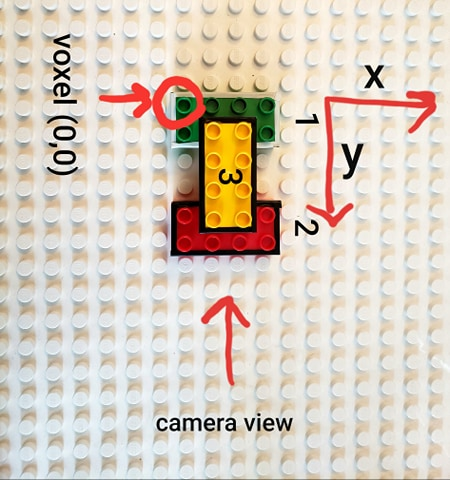
\includegraphics[width = 0.8\textwidth]{figures/voxel_3objs.jpg}
   \caption[{Attributes of \emph{Assembly\_Graph} and \emph{Block} explained}]{Attributes of \emph{Assembly\_Graph} and \emph{Block} explained: The reference voxel (0,0) is circled in red. Green block has .idx $=1$, red block has .idx $= 2$ and yellow block has .idx $= 3$. Green and red blocks are at 90 degrees angle and yellow is at 0 degrees. Green and red blocks need to be placed before yellow block. Yellow block is the only block that can be removed in the next action.}
   \label{fig:fig_3-2}
\end{figure}

For teaching mode, class \textbf{Assembly\_Graph}, has an extra attribute of type \textbf{Assembly\_Graph} to pass the target dictionary that is saved in learning mode. Using these attributes various functions are defined within the class to add and remove blocks, save and load the model, display the model and compare the models to flag errors. Feedback selection and passing the feedback statement to robot is done using functions within this class as well. 

\subsect{Processing Pipeline}
Figure \ref{fig:fig_3-3} shows the work flow of the system for both modes. The RealSense\textsuperscript\textregistered{} d435i camera captures and provides a continuous RGB-D images stream. First of all, the reference block is added to the model giving (0,0) coordinates for \textbf{.xy} of class \emph{Block} as described above. Once that is done successfully, the system scans for control command in three control boxes: add, remove and adjust. As soon as a block is detected in one of the control boxes, the system processes the play area for requisite action and updates the model accordingly. If system is in learning mode, on completion of required action, the system again scans for new action and the cycle continues till program is exited. If system is in teaching mode, on completion of requested action, the system compares the current action with all possible correct actions (comparison is made on add and adjust commands and not on remove command) and forwards the errors with respect to every possible correct action to the feedback module. The feedback module chooses a message based on errors and feedback strategy which is published for the robot to convey to the user. Once this action is completed, system starts scanning the control boxes again for next action request. The system exists when the current model is same as target model. In the following sections, we describe details of how each step in the workflow is accomplished. 
% Figure 3-3
\begin{figure}[h]
    \begin{subfigure}{1\textwidth}
       \centering
    %   \includegraphics[width=\textwidth,height=\textheight,keepaspectratio]{fig_3-3}
       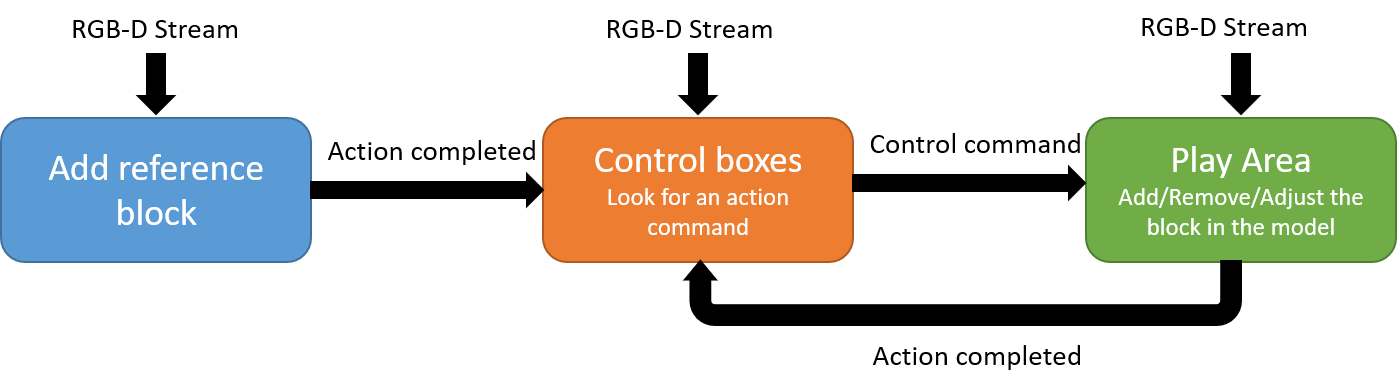
\includegraphics[width=1\linewidth]{figures/learning_mode.png}
      
       \caption[{Learning mode}]{ \label{fig:fig_3-3a}}
    \end{subfigure}
    \begin{subfigure}{1\textwidth}
       \centering
    %   \includegraphics[width=\textwidth,height=\textheight,keepaspectratio]{fig_3-3}
       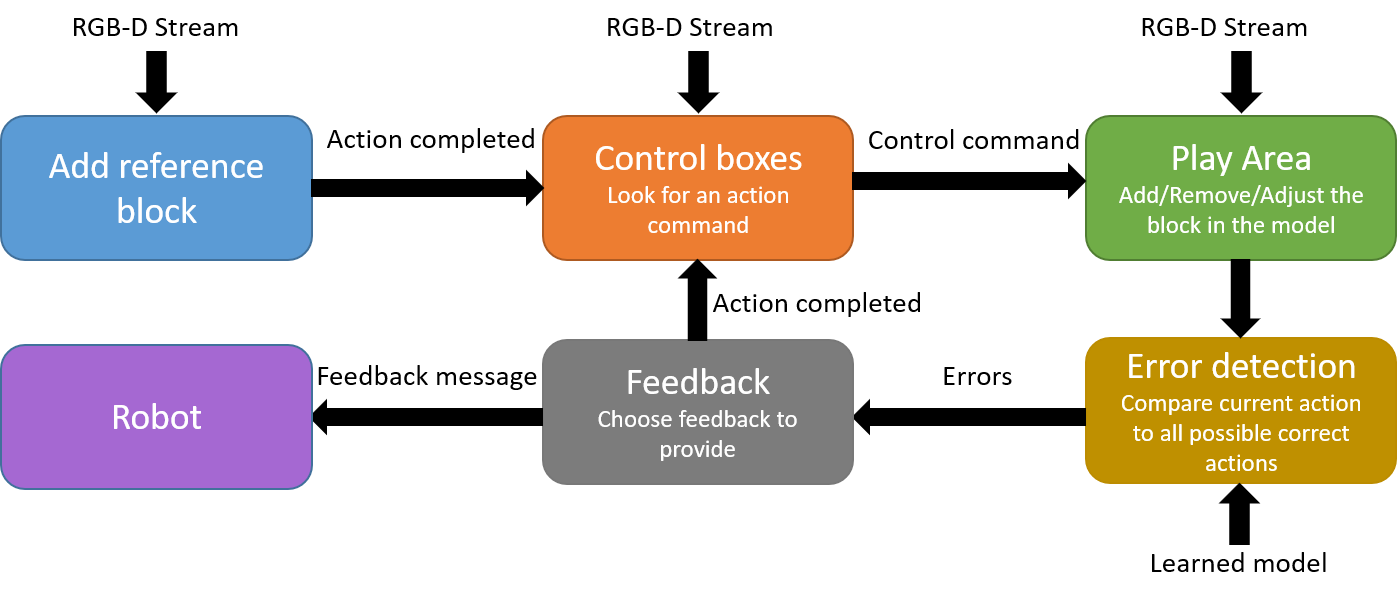
\includegraphics[width=1\linewidth]{figures/teaching_mode.png}
      
       \caption[{Teaching mode}]{ \label{fig:fig_3-3b}}
    \end{subfigure}
    \caption[{Processing pipeline}]{Processing pipeline for perception module (a) for learning mode (b) for teaching mode}
   \label{fig:fig_3-3}
\end{figure}
\subsect{Scanning Control Boxes}
The continuous RGB image stream is divided into 4 fixed regions: add box, remove box, adjust box and play area. The add, remove and adjust boxes are scanned for next command after reference block is added. The RGB image from each box is segmented using Hue, Saturation, and Value (HSV) based color segmentation to create a binary mask for each of the four colors (red, green, blue and yellow). Bounding rectangle is found for largest contour in the mask by using builtin functions of openCV (findContous(arguments), max(arguments) and boundingRect(arguments)). If a bounding rectangle is found for same color in same control box for 50 consecutive frames, it is considered a control command. The color and shape (assigned by looking at width to height ratio of the bounding rectangle) of the new block is noted, the respective command (add, remove or adjust) is activated and system starts scanning play area.
\subsect{Scanning Play Area}
RGB-D continuous stream is scanned for new action as per the control command. For  add action, first of all, the RGB image is segmented using HSV based color segmentation to create binary mask of color of new block (color is known from control command). Now, this mask is compared with masks from previous frames and if there is no change in the mask for n of consecutive frames (n= 50 for our system), all contours whose bounding boxes have width of more than m pixels (m = 15 for our system) and have the same shape as indicated by control box are considered as \emph{possible additions}. The x and y pixel coordinates of the center of each bounding box is used to get depth (z) from the corresponding depth data. If the block is $2 \times 4$ block, angle is calculated for each possible addition using ratio of width to height of the bounding box. Next, all the \emph{possible additions} are compared with the existing blocks in the model (x,y,z, shape, color and angle). The contours that coincide with existing blocks in the model are discarded thus leaving us with the contour of new block. This block is then added to the model by passing its attributes (x,y,z,shape, color, angle). The system keeps scanning the play area for new block till a block is added in the model. Once the block is added, the system generates a flag indicating that the add action is completed. For learning mode, each time new block is added \textbf{.idx} is counted up. For teaching mode, if the new block added in the current model matches one of the blocks in target model, \textbf{.idx} of the new block in the current model is assigned the same value as in target model otherwise it is assigned a much higher value e.g. 21, 22, 23. This makes comparison of two models efficient and easy. \\
For remove action, mask of known color is created using HSV based color segmentation and is compared with previous frames till there is no change for n consecutive frames (n = 50 for our system). Contours with bounding boxes are calculated. From the model, using a function \textbf{.removable\_blocks()}, we can get the \textbf{.idx} of all the blocks that can be removed from the current dictionary. We can also get the \textbf{.idx} of blocks in the model of the shape and color associated with the remove command. Intersection of these two lists, will give us \emph{possible removable blocks} i.e. the \textbf{.idx} of the blocks that are removable and of given specifications from remove command. If it is only one block that lies at intersection of these two lists, we remove that block from the model. If there are multiple blocks that can be removed, we look at the bounding boxes of contours of known shape and check which blocks from the model are still in the play area by comparing x, y, z and angle of the contours to the blocks in the model. Discard the \textbf{.idx} of these blocks from \emph{possible removable blocks} as these are still present in the play area. There should only be one block left behind in list of \emph{possible removable blocks}, which is the one that has been removed from the play area and placed in the remove box. System generates a flag indicating that the action is completed successfully when the block is removed from the model. Remove action is same for both learning and teaching mode. \\
For adjust action, remove action is completed followed by add action for the block detected in adjust box. System generates a flag on completion of action and starts scanning for next action. 
\subsect{Types of Errors Detected}
Following types of errors are detected for new block to be added in comparison to all possible correct blocks and passed to feedback module:
\begin{enumerate}
    \item Shape: The shape of new block is different from the possible correct block.
    \item Color: The color of new block is different from the possible correct block.
    \item Orientation: The orientation of new block is different from the possible correct block.
    \item Level: The \textbf{.z} (z-level) of new block is different from the possible correct block.
    \item Position: The center of new block is different from the possible correct block.
\end{enumerate}


% Figure 3-6
\begin{figure}[H]
    \begin{subfigure}{0.5\textwidth}
       \centering
    %   \includegraphics[width=\textwidth,height=\textheight,keepaspectratio]{fig_3-3}
       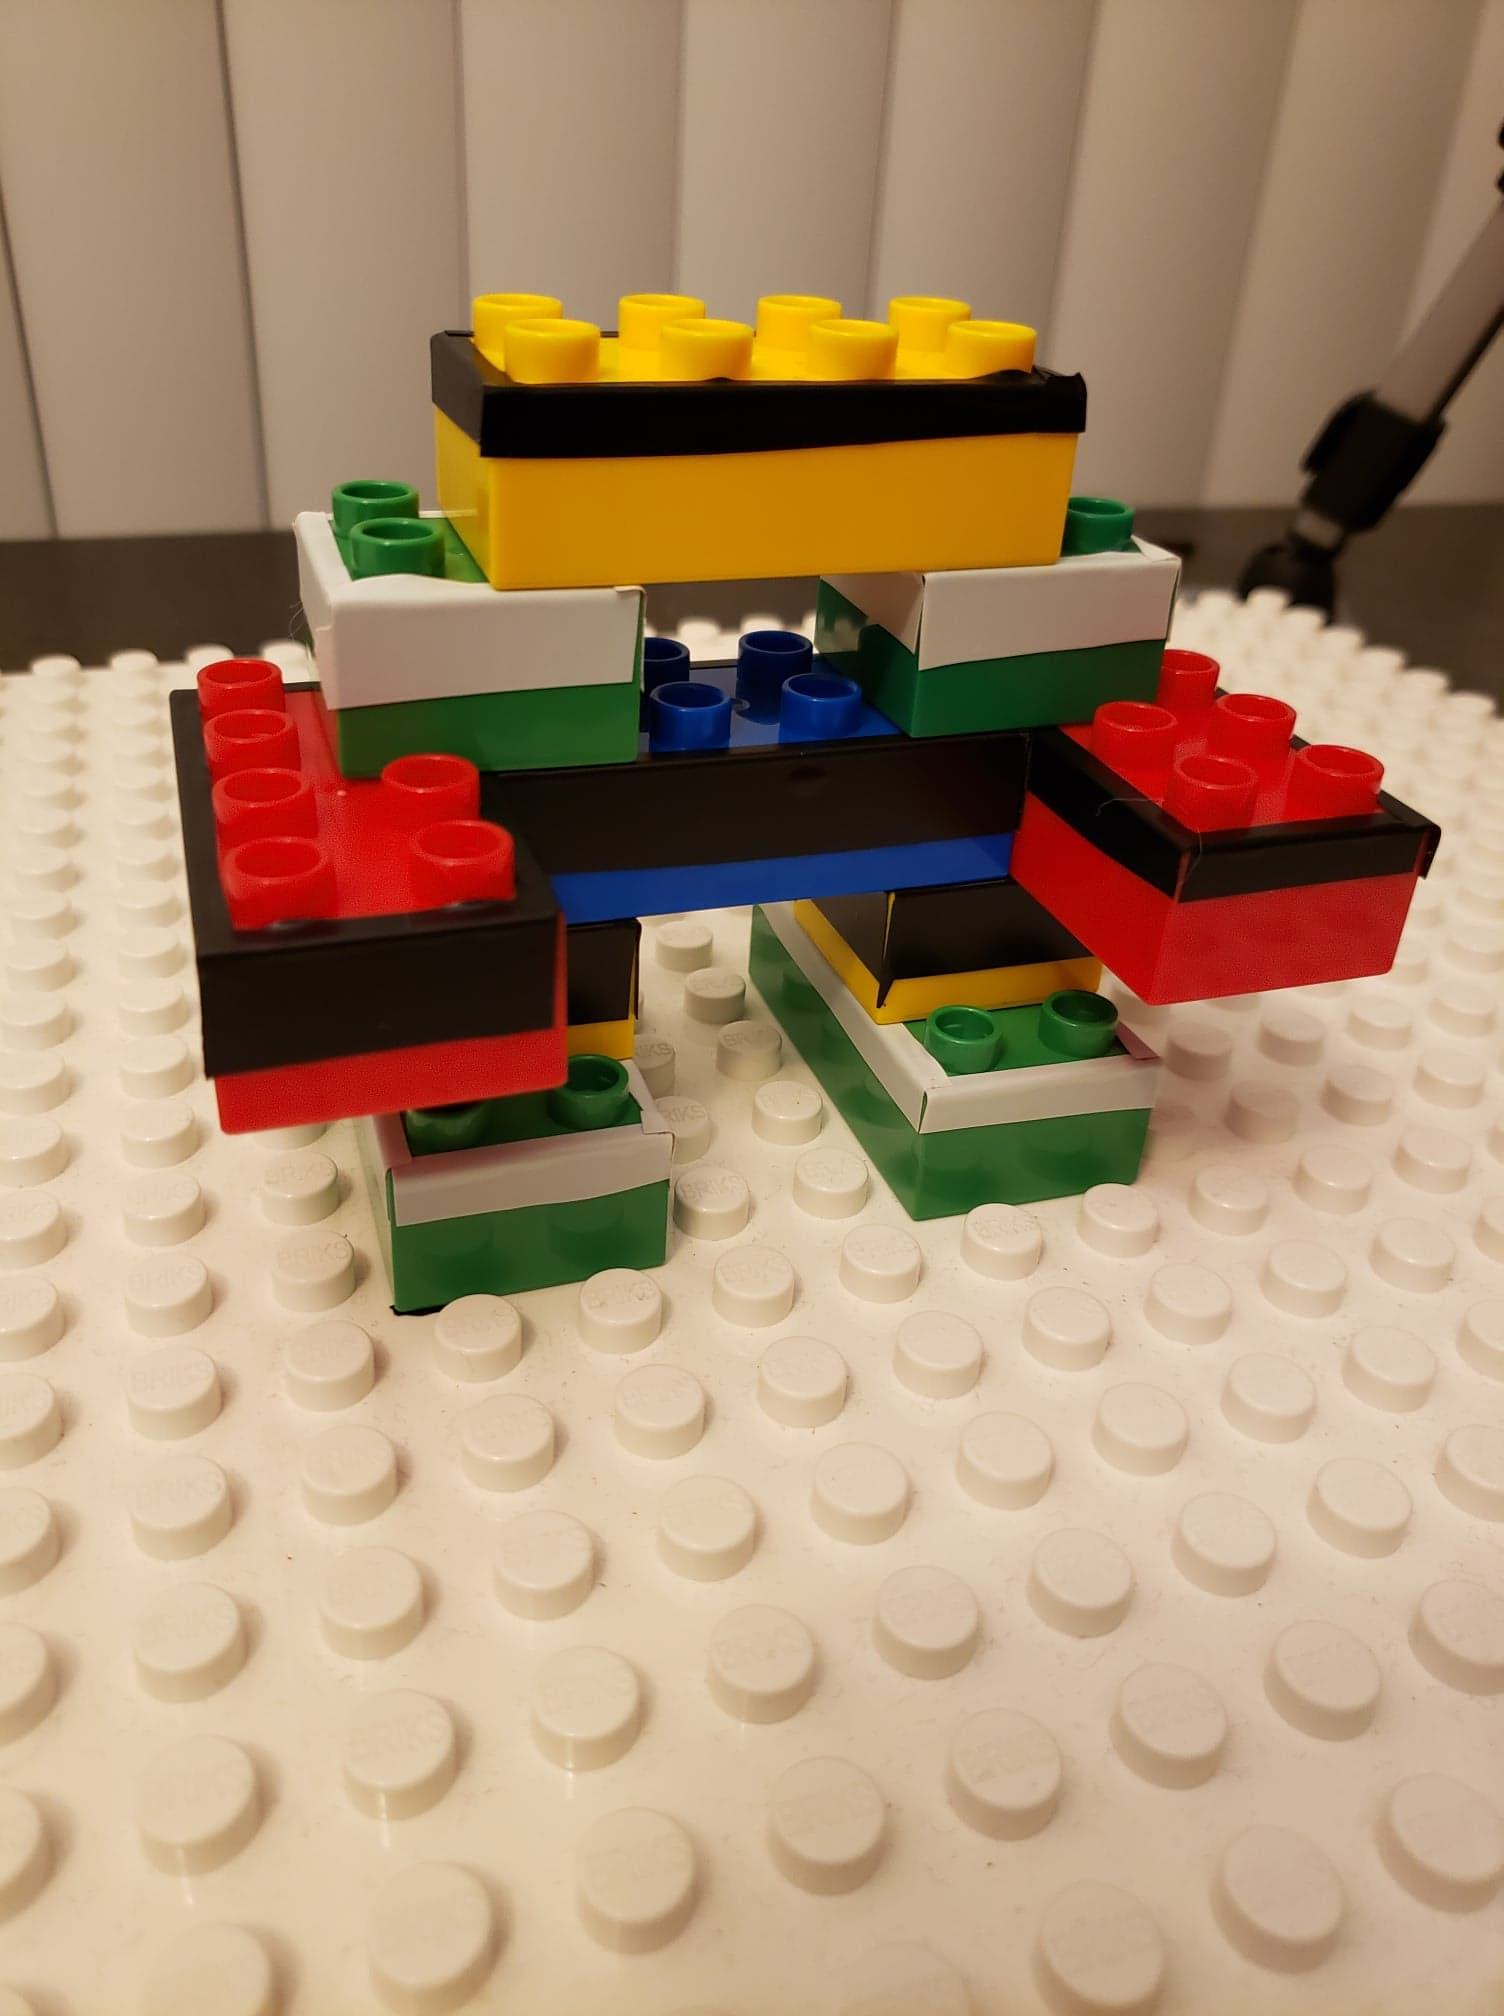
\includegraphics[width=0.8\linewidth,trim={0 25cm 0 5cm},clip]{figures/t1.jpg}
       
       \caption[{}]{\label{fig:fig_3-6a}}
    \end{subfigure}
    \begin{subfigure}{0.5\textwidth}
       \centering
    %   \includegraphics[width=\textwidth,height=\textheight,keepaspectratio]{fig_3-3}
       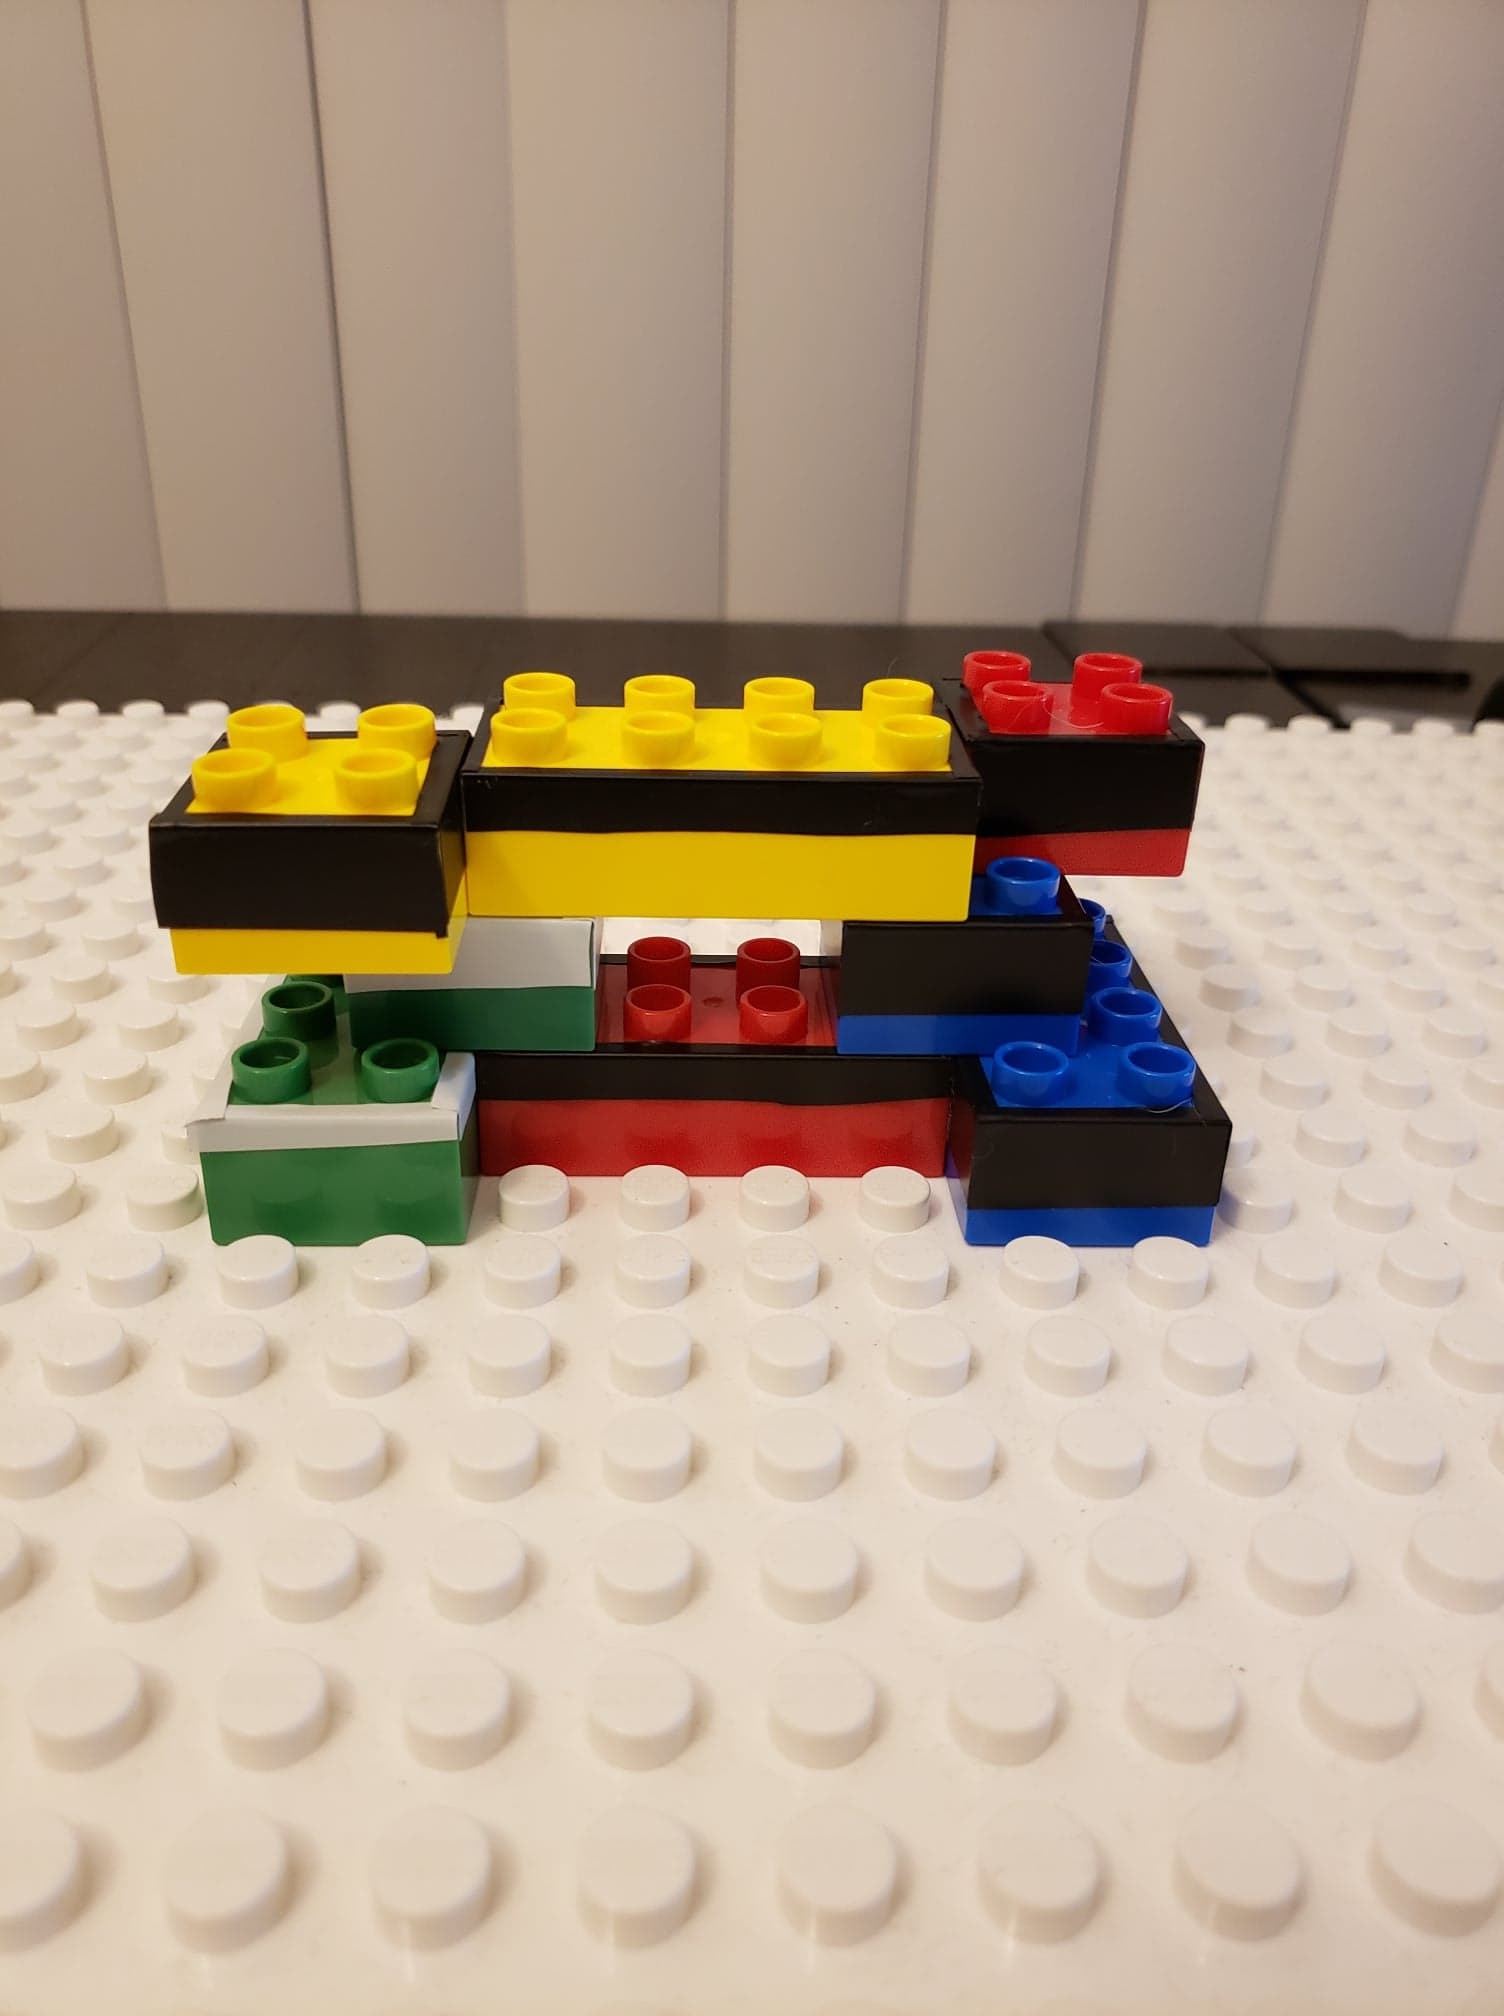
\includegraphics[width=0.8\linewidth,trim={0 20cm 0 10cm},clip]{figures/t2.jpg}
       
       \caption[{}]{\label{fig:fig_3-6b}}
    \end{subfigure}
    \begin{subfigure}{0.5\textwidth}
       \centering
    %   \includegraphics[width=\textwidth,height=\textheight,keepaspectratio]{fig_3-3}
       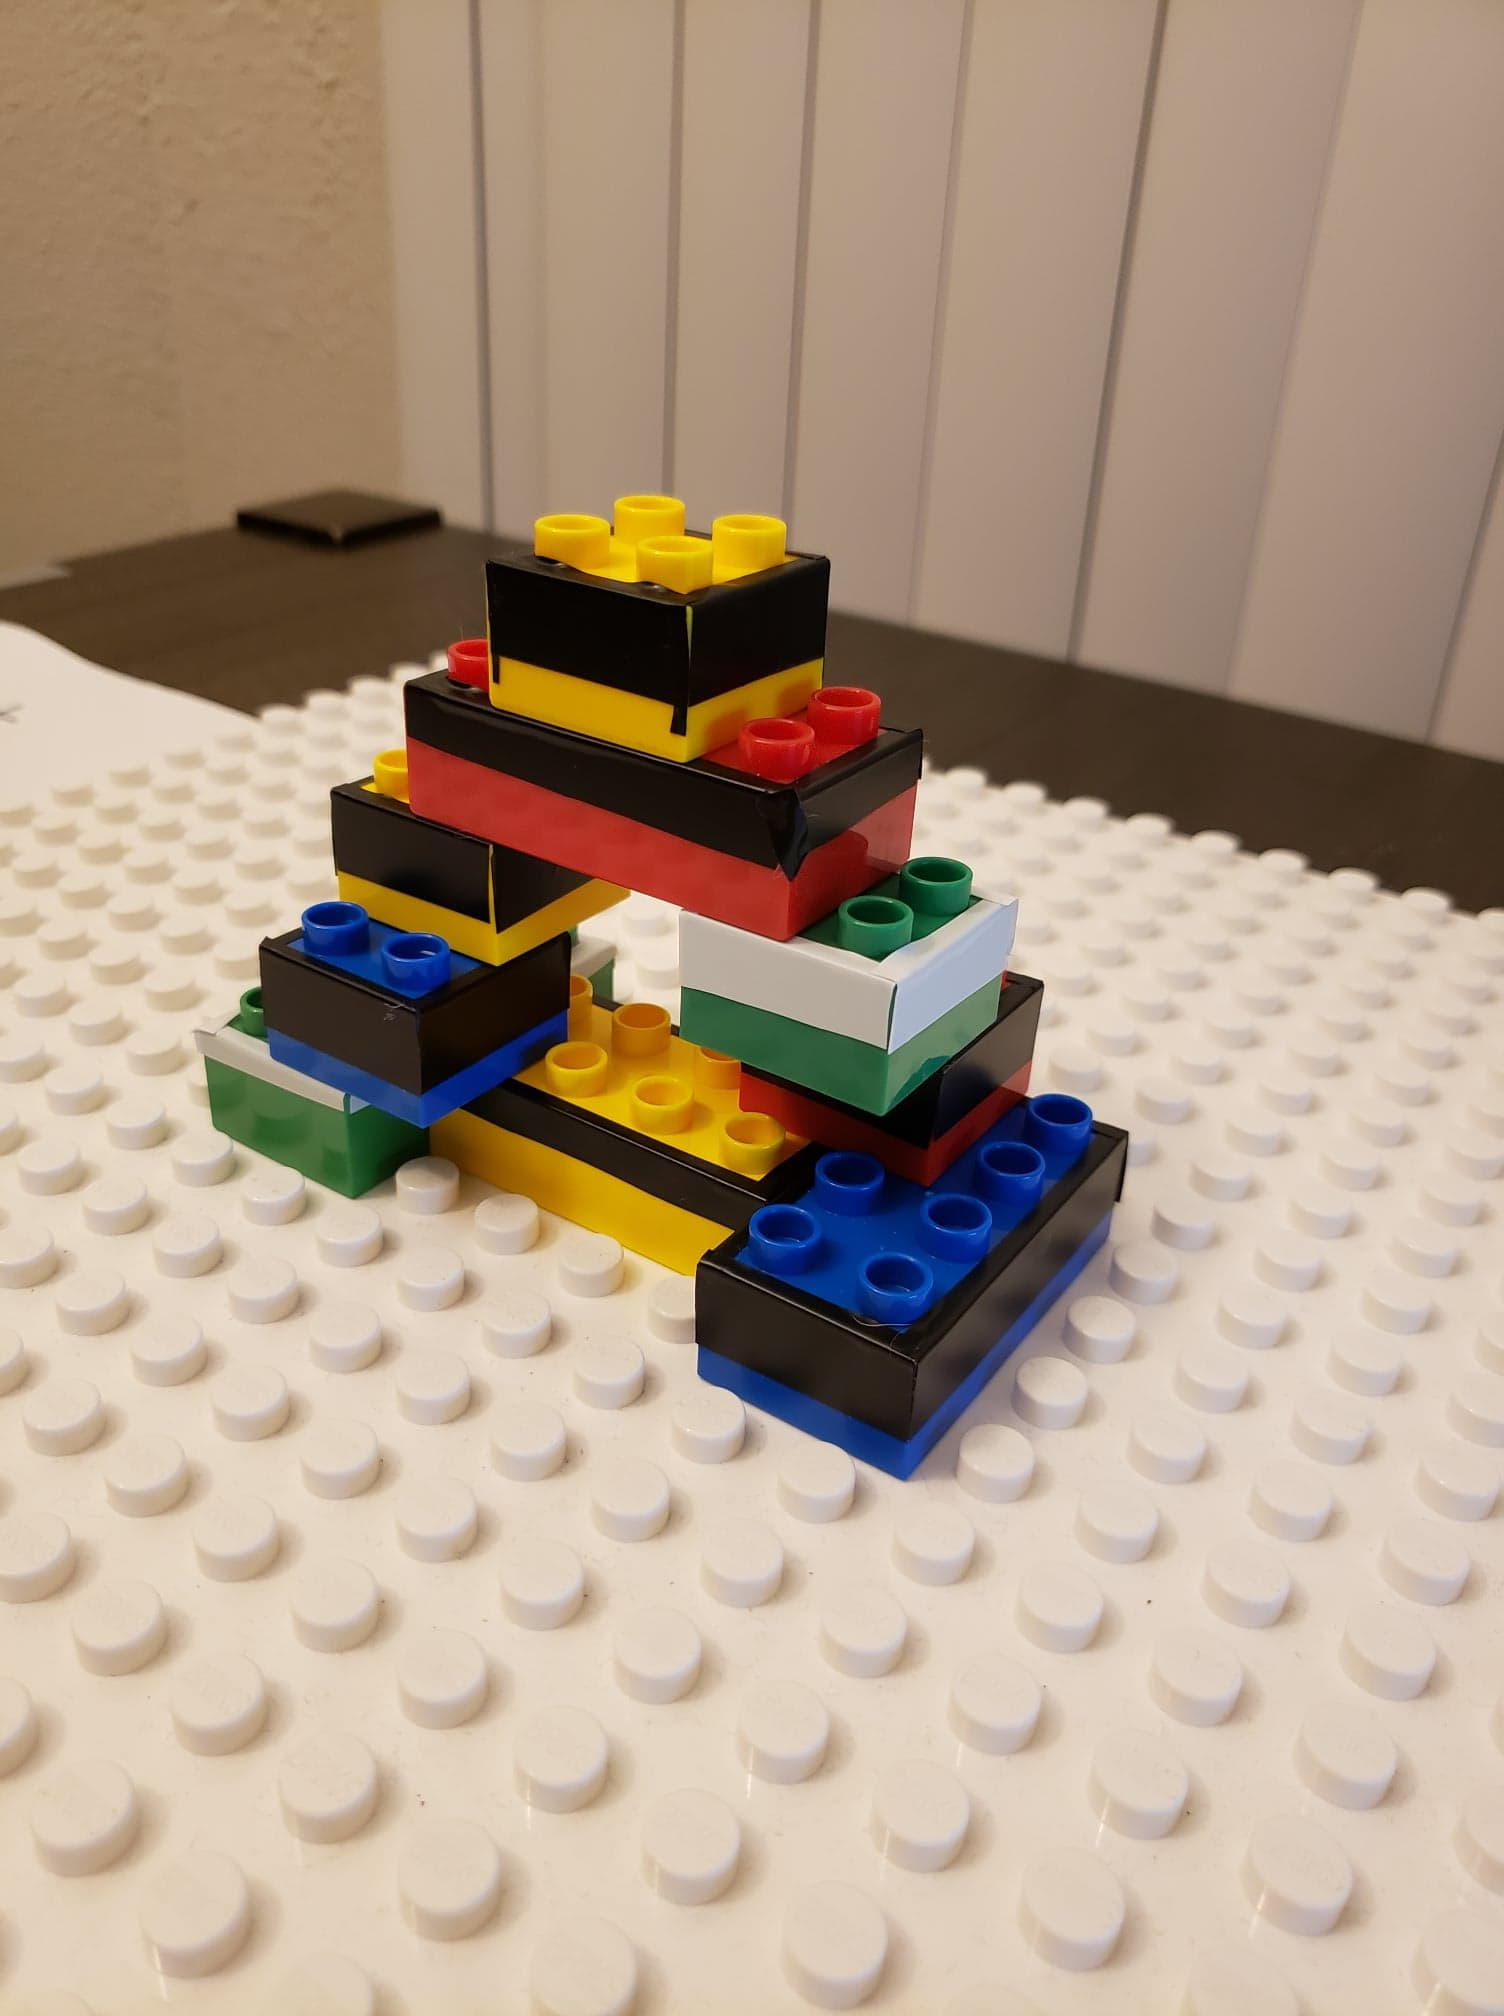
\includegraphics[width=0.8\linewidth,trim={0 15cm 0 15cm},clip]{figures/t3.jpg}
       
       \caption[{}]{\label{fig:fig_3-6c}}
    \end{subfigure}
    \begin{subfigure}{0.5\textwidth}
       \centering
    %   \includegraphics[width=\textwidth,height=\textheight,keepaspectratio]{fig_3-3}
       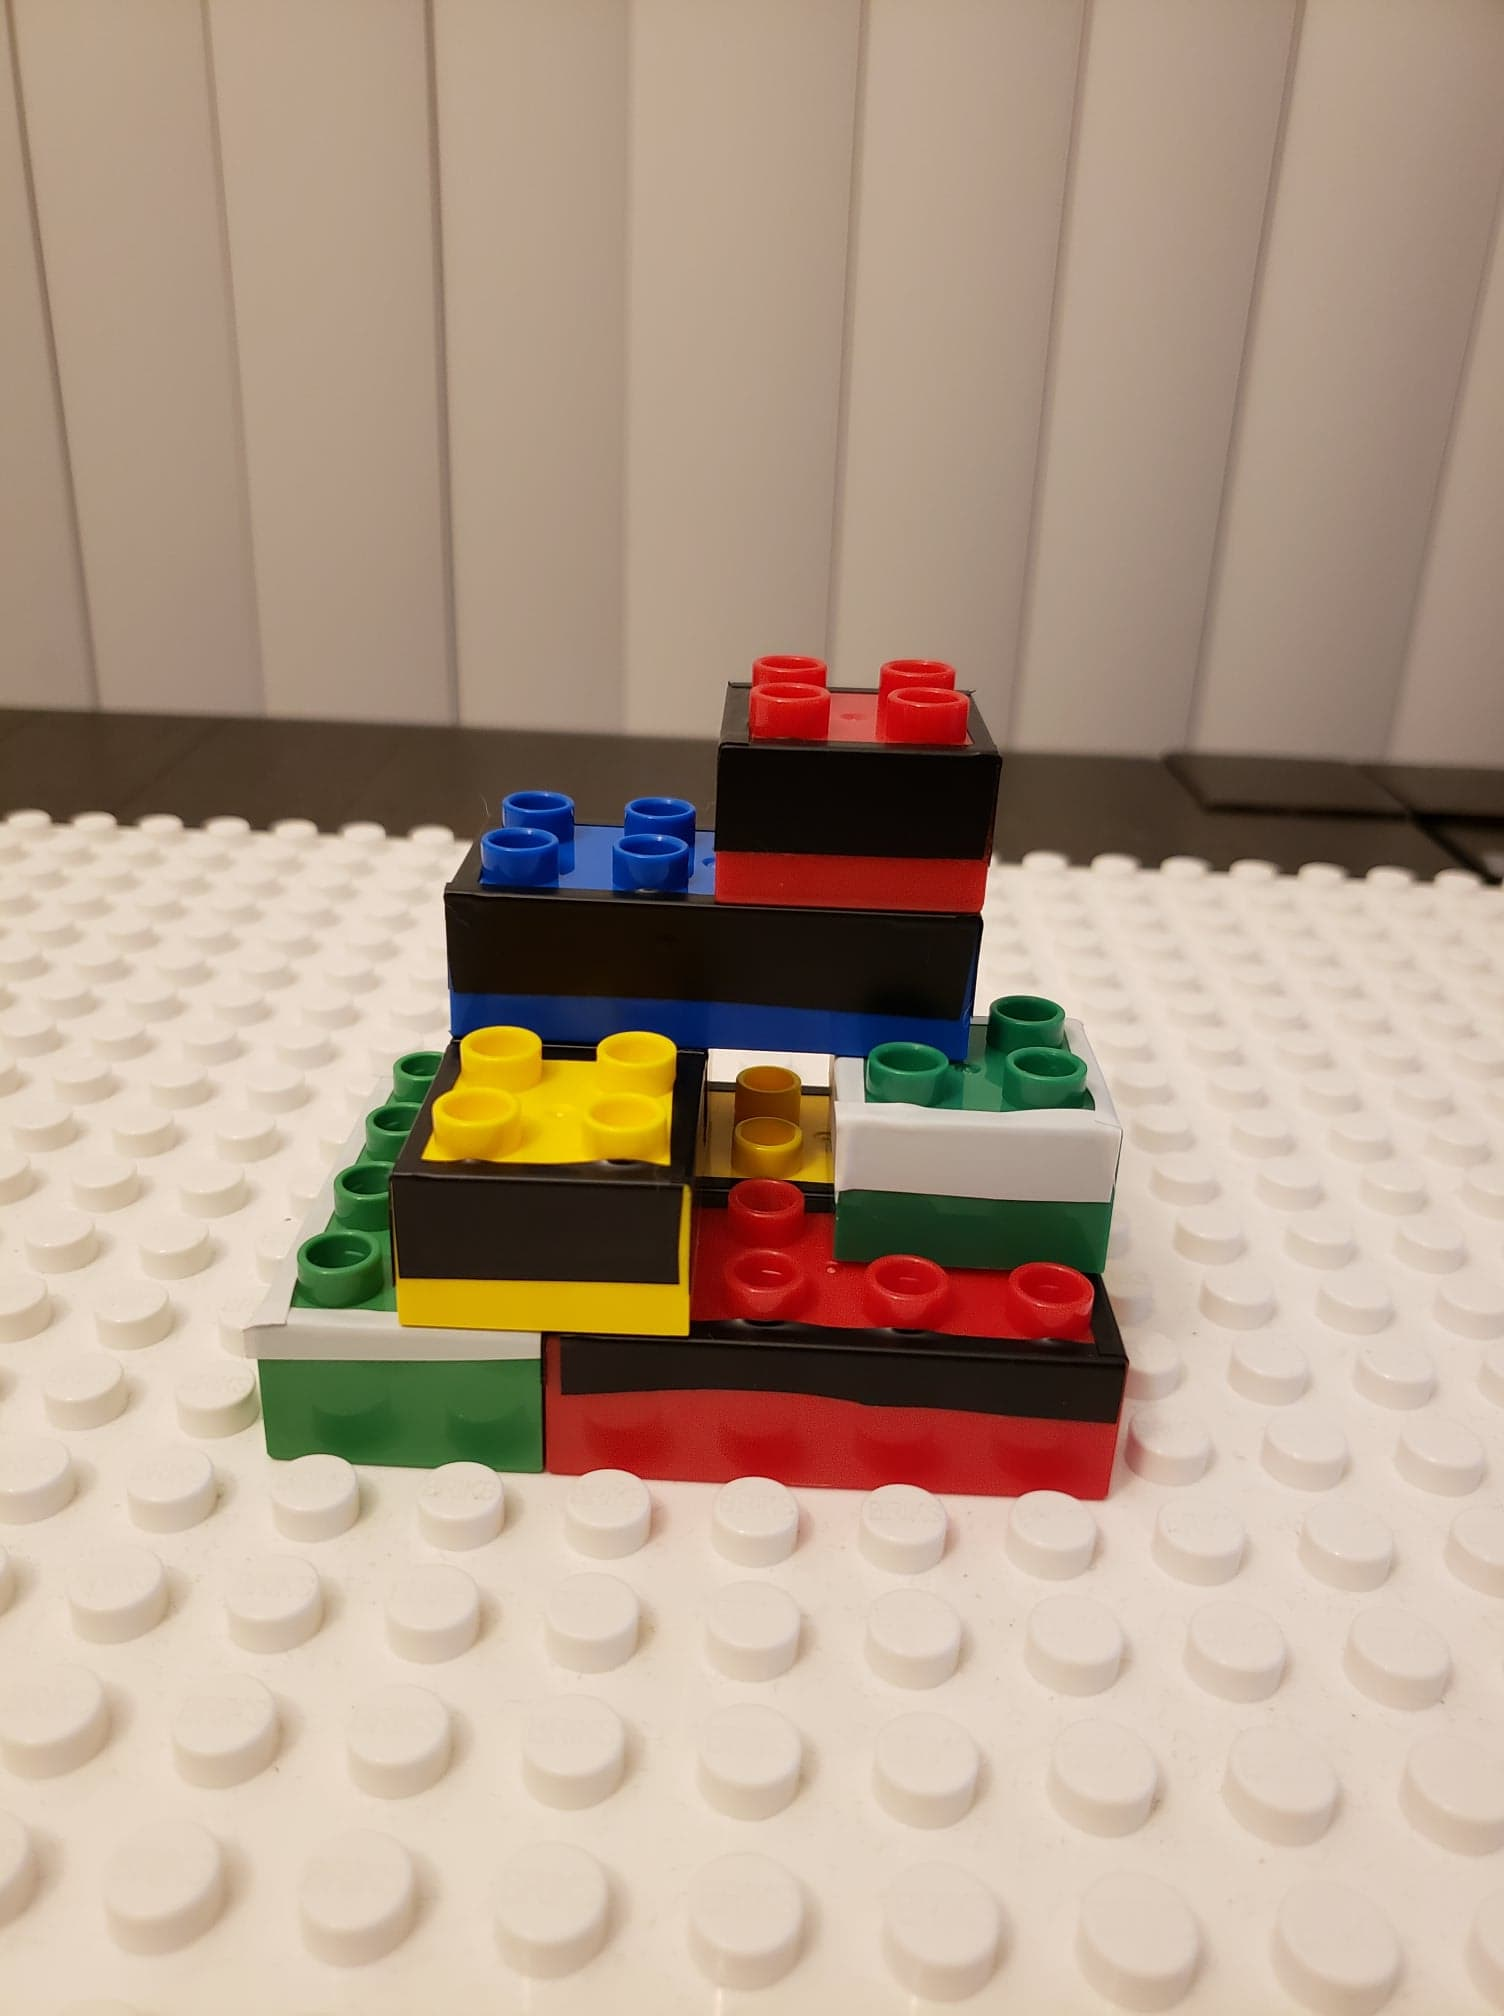
\includegraphics[width=0.8\linewidth,trim={0 15cm 0 15cm},clip]{figures/t4.jpg}
       
       \caption[{}]{\label{fig:fig_3-6d}}
    \end{subfigure}
    \begin{subfigure}{0.5\textwidth}
       \centering
    %   \includegraphics[width=\textwidth,height=\textheight,keepaspectratio]{fig_3-3}
       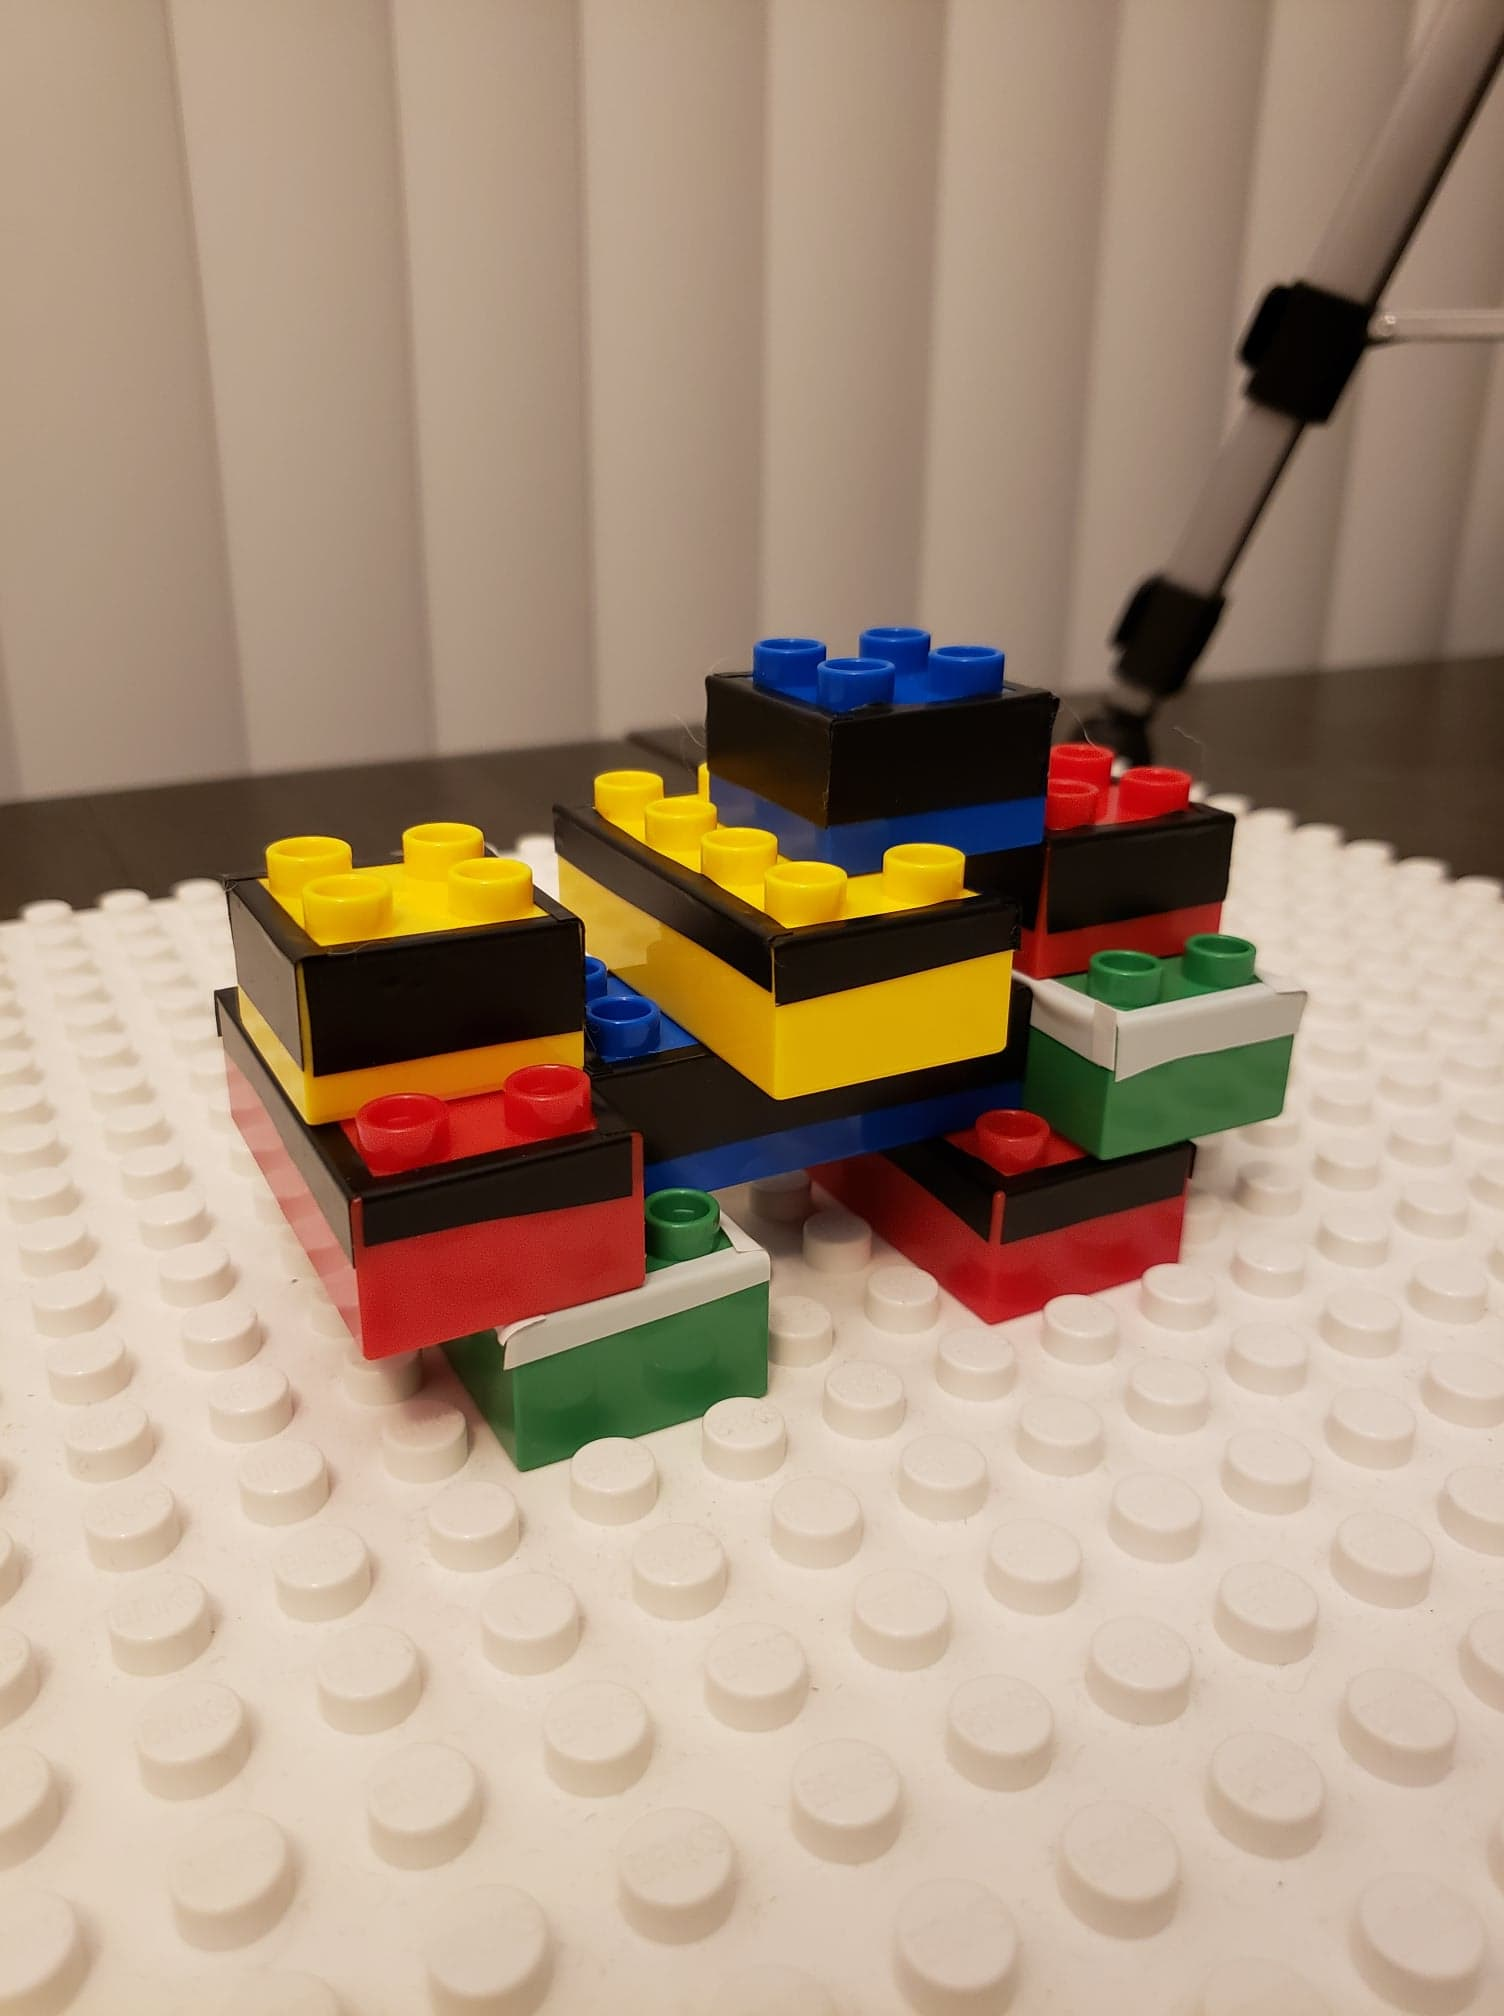
\includegraphics[width=0.8\linewidth,trim={0 10cm 0 20cm},clip]{figures/t6.jpg}
      
       \caption[{}]{ \label{fig:fig_3-6e}}
    \end{subfigure}
    \begin{subfigure}{0.5\textwidth}
       \centering
    %   \includegraphics[width=\textwidth,height=\textheight,keepaspectratio]{fig_3-3}
       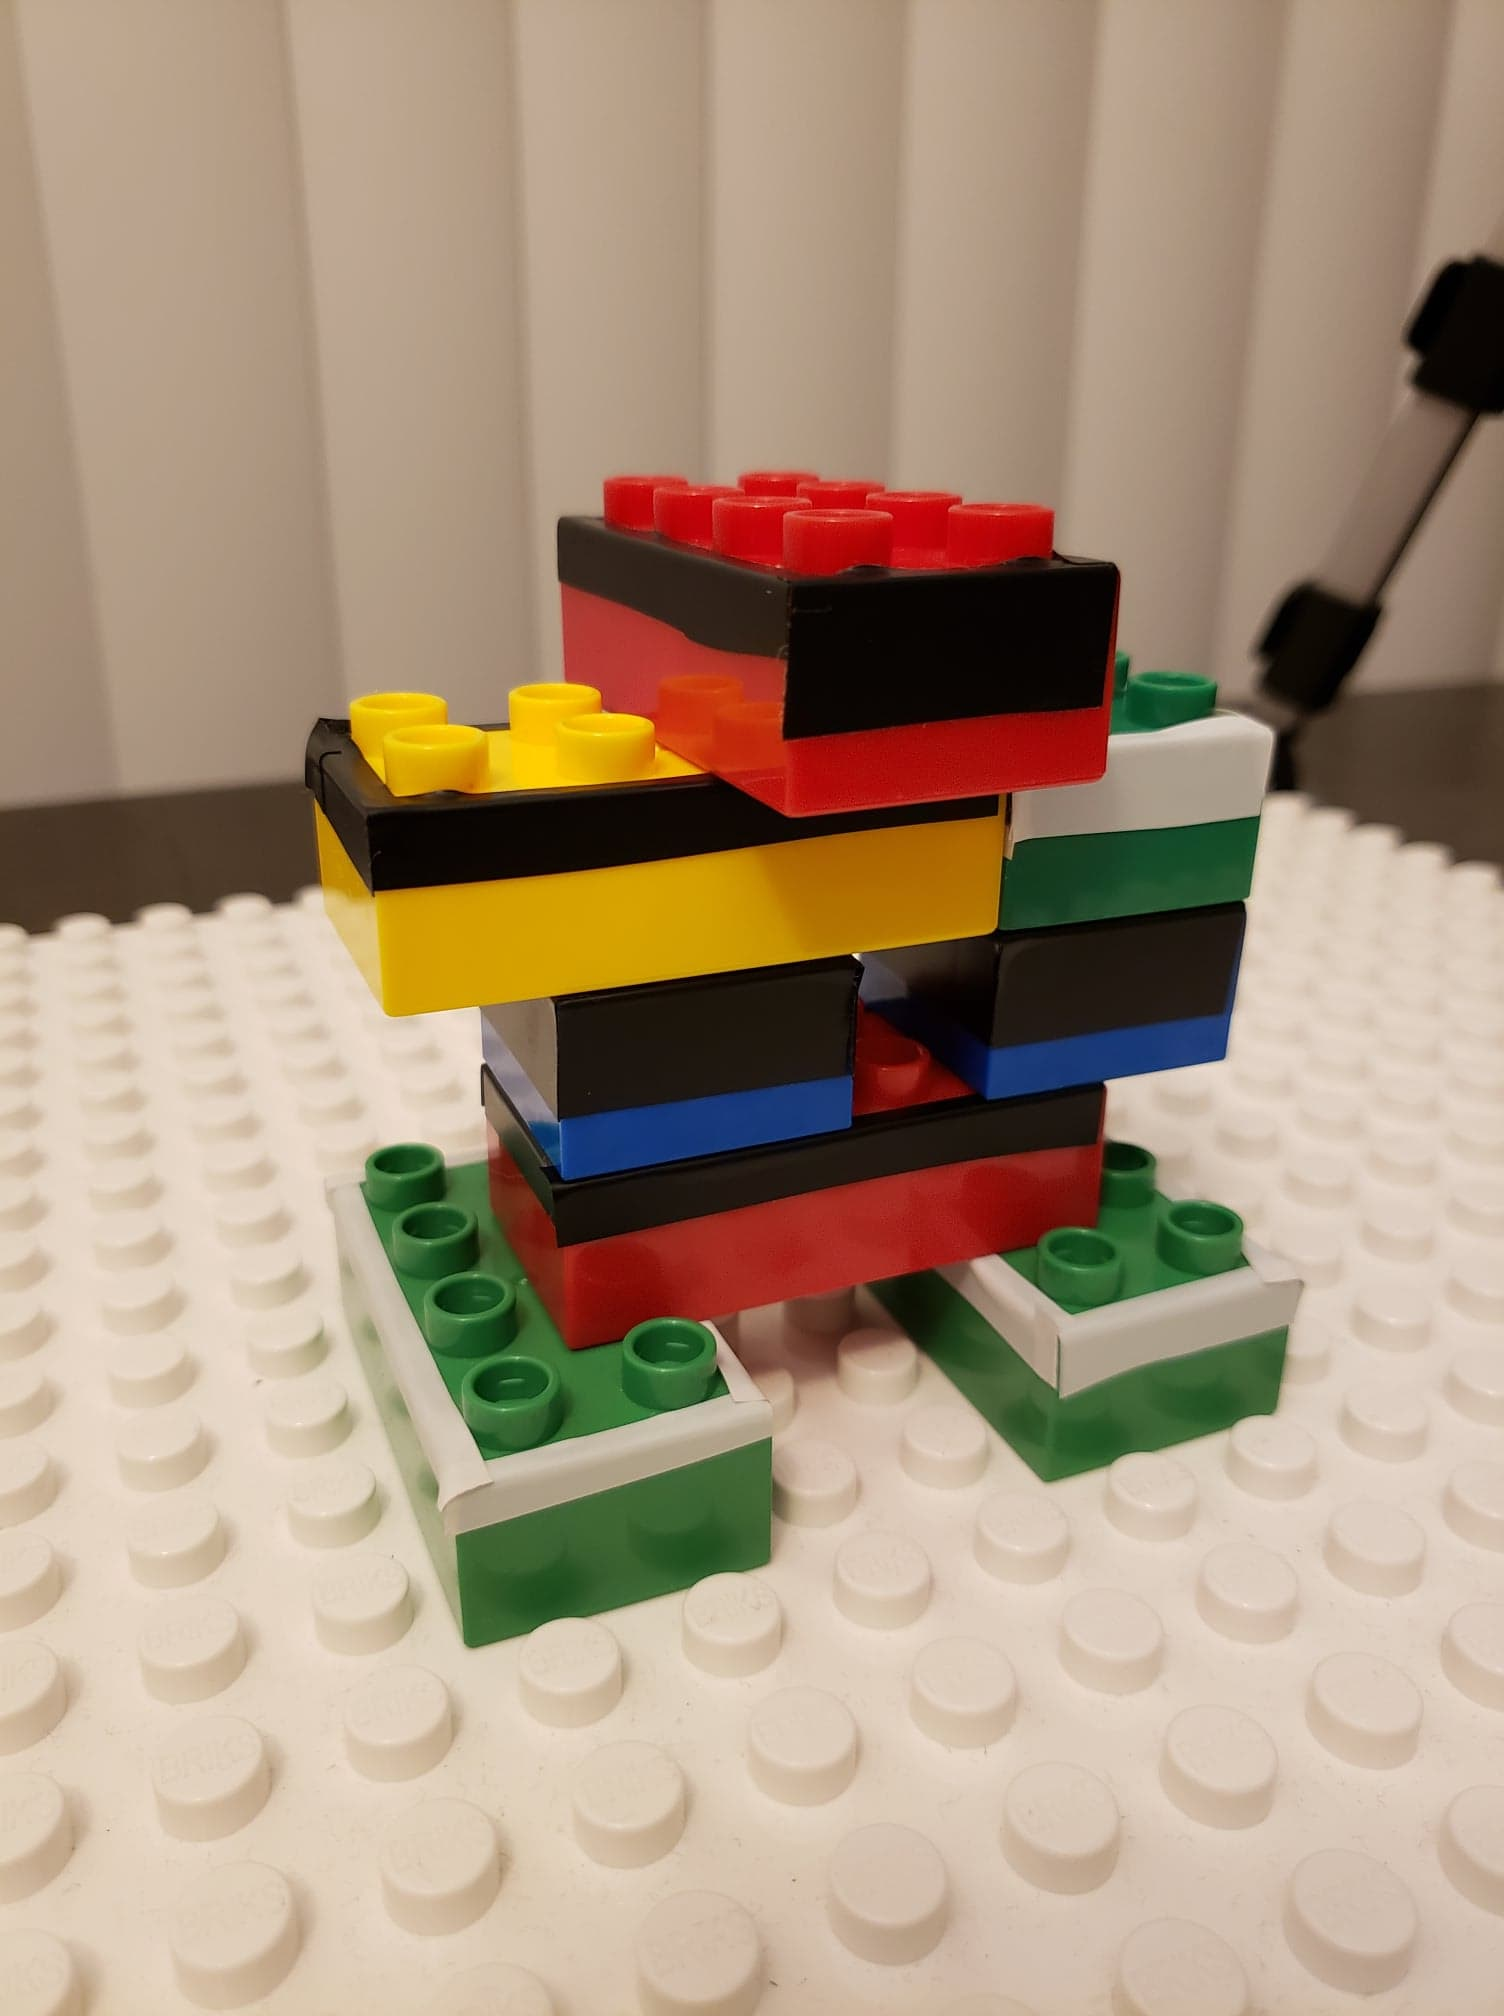
\includegraphics[width=0.8\linewidth,trim={0 15cm 0 15cm},clip]{figures/t7.jpg}
       
       \caption[{}]{\label{fig:fig_3-6f}}
    \end{subfigure}
    \begin{subfigure}{0.5\textwidth}
       \centering
    %   \includegraphics[width=\textwidth,height=\textheight,keepaspectratio]{fig_3-3}
       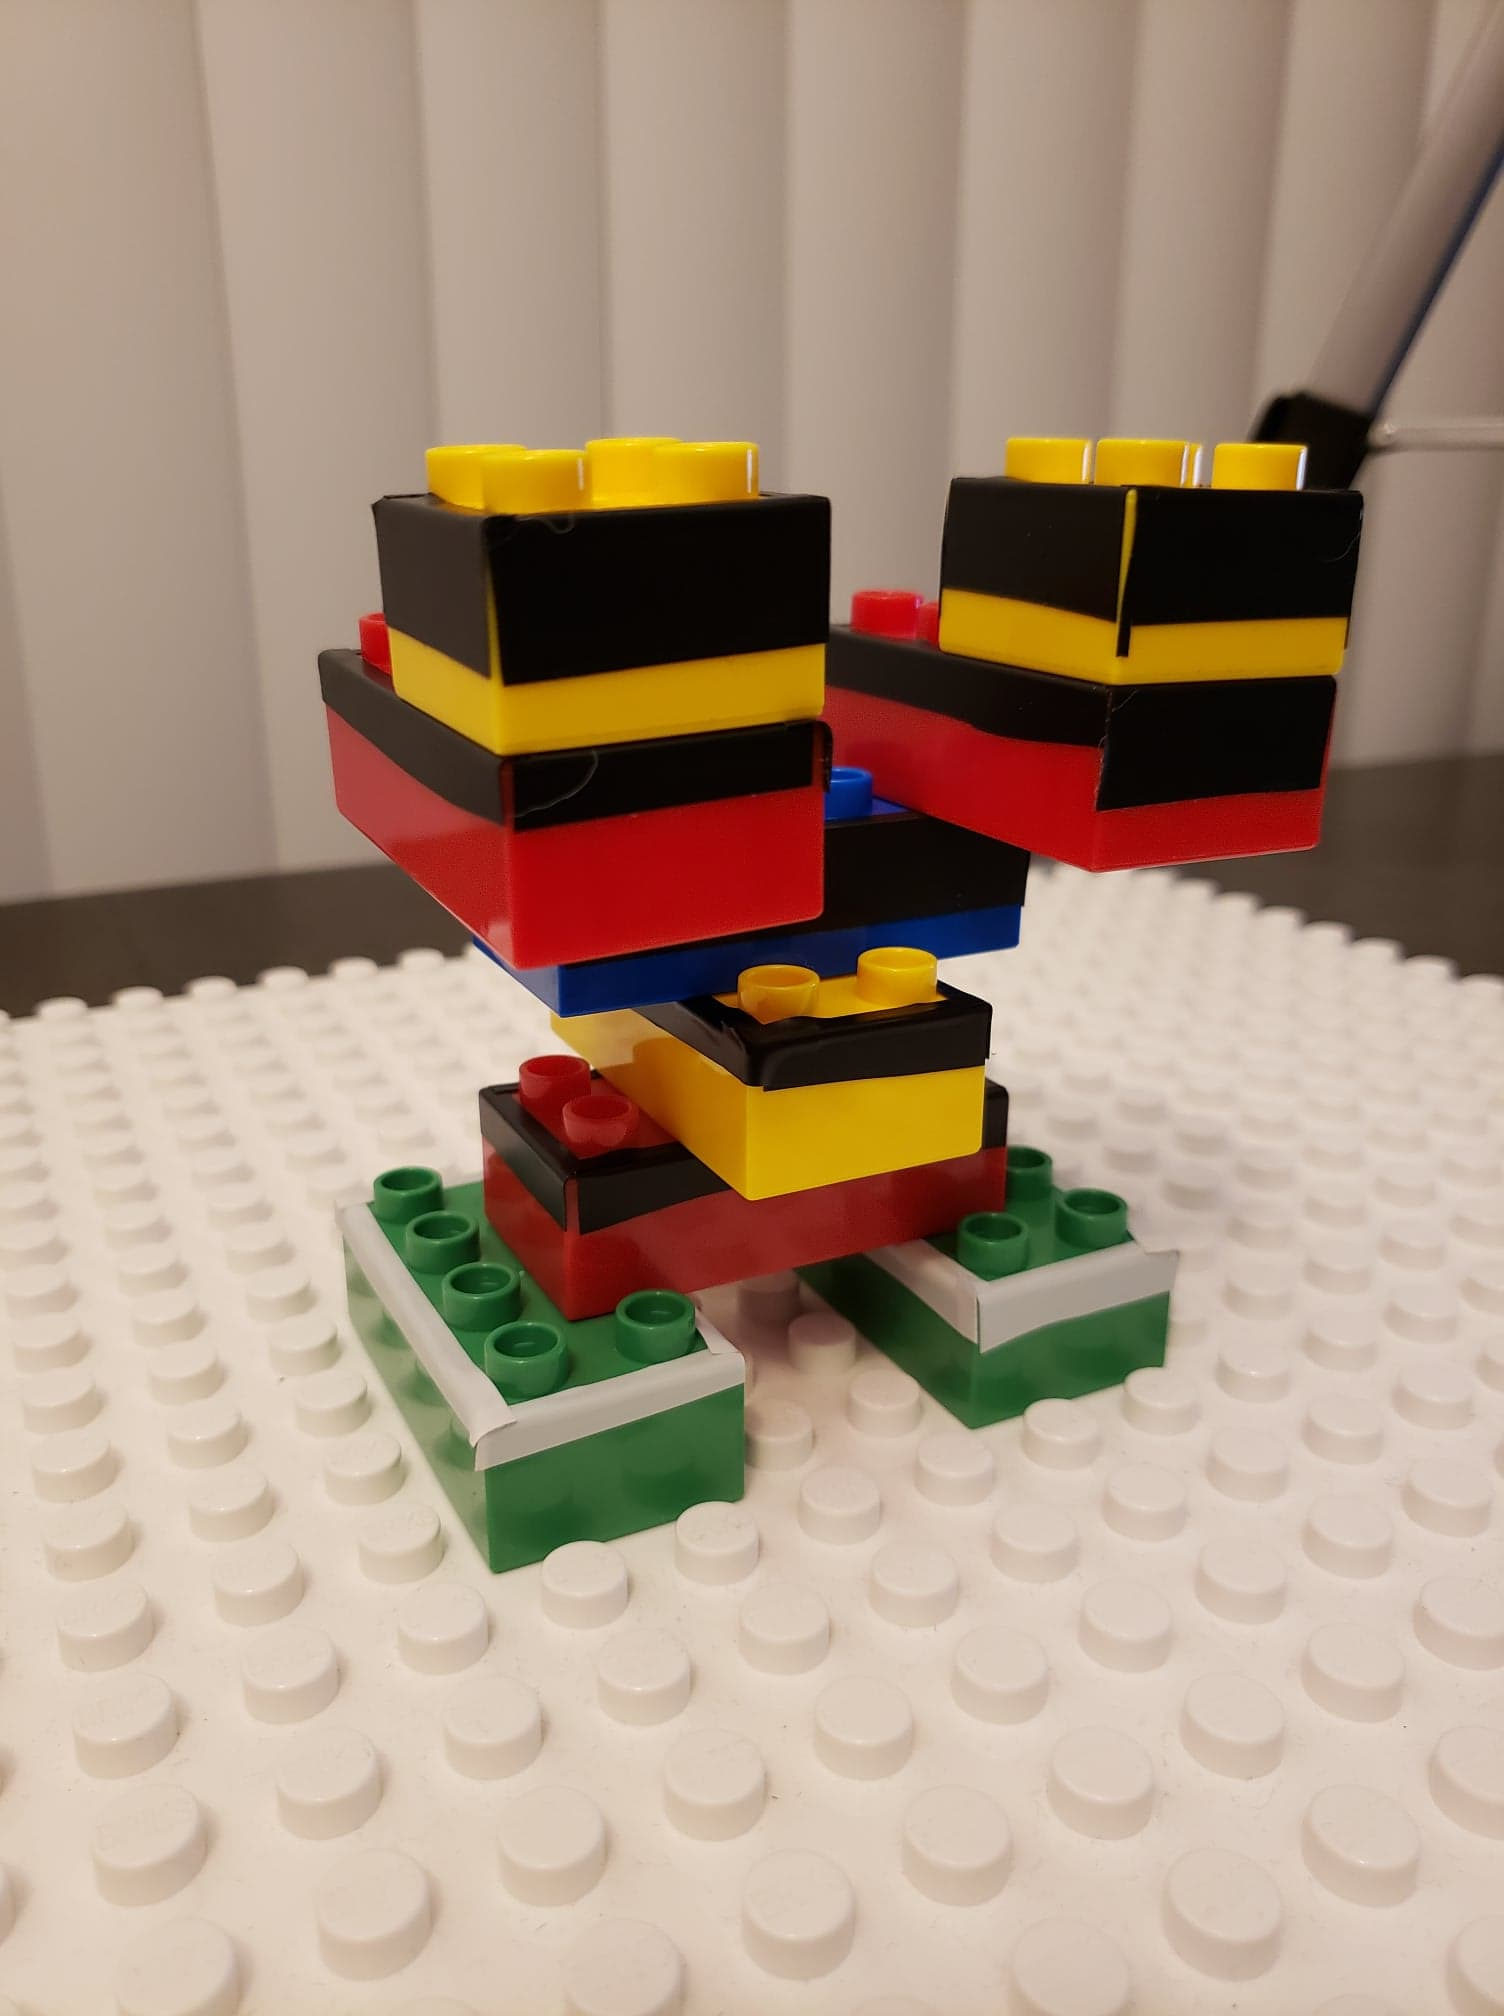
\includegraphics[width=0.8\linewidth,trim={0 15cm 0 15cm},clip]{figures/t5.jpg}
      
       \caption[{}]{ \label{fig:fig_3-6g}}
    \end{subfigure}
    \caption[{Simple 3D structures}]{Simple 3D structures successfully completed in both learning and teaching modes.}
   \label{fig:fig_3-6}
\end{figure}
% Figure 3-7
\begin{figure}[H]
    \begin{subfigure}{0.5\textwidth}
       \centering
    %   \includegraphics[width=\textwidth,height=\textheight,keepaspectratio]{fig_3-3}
       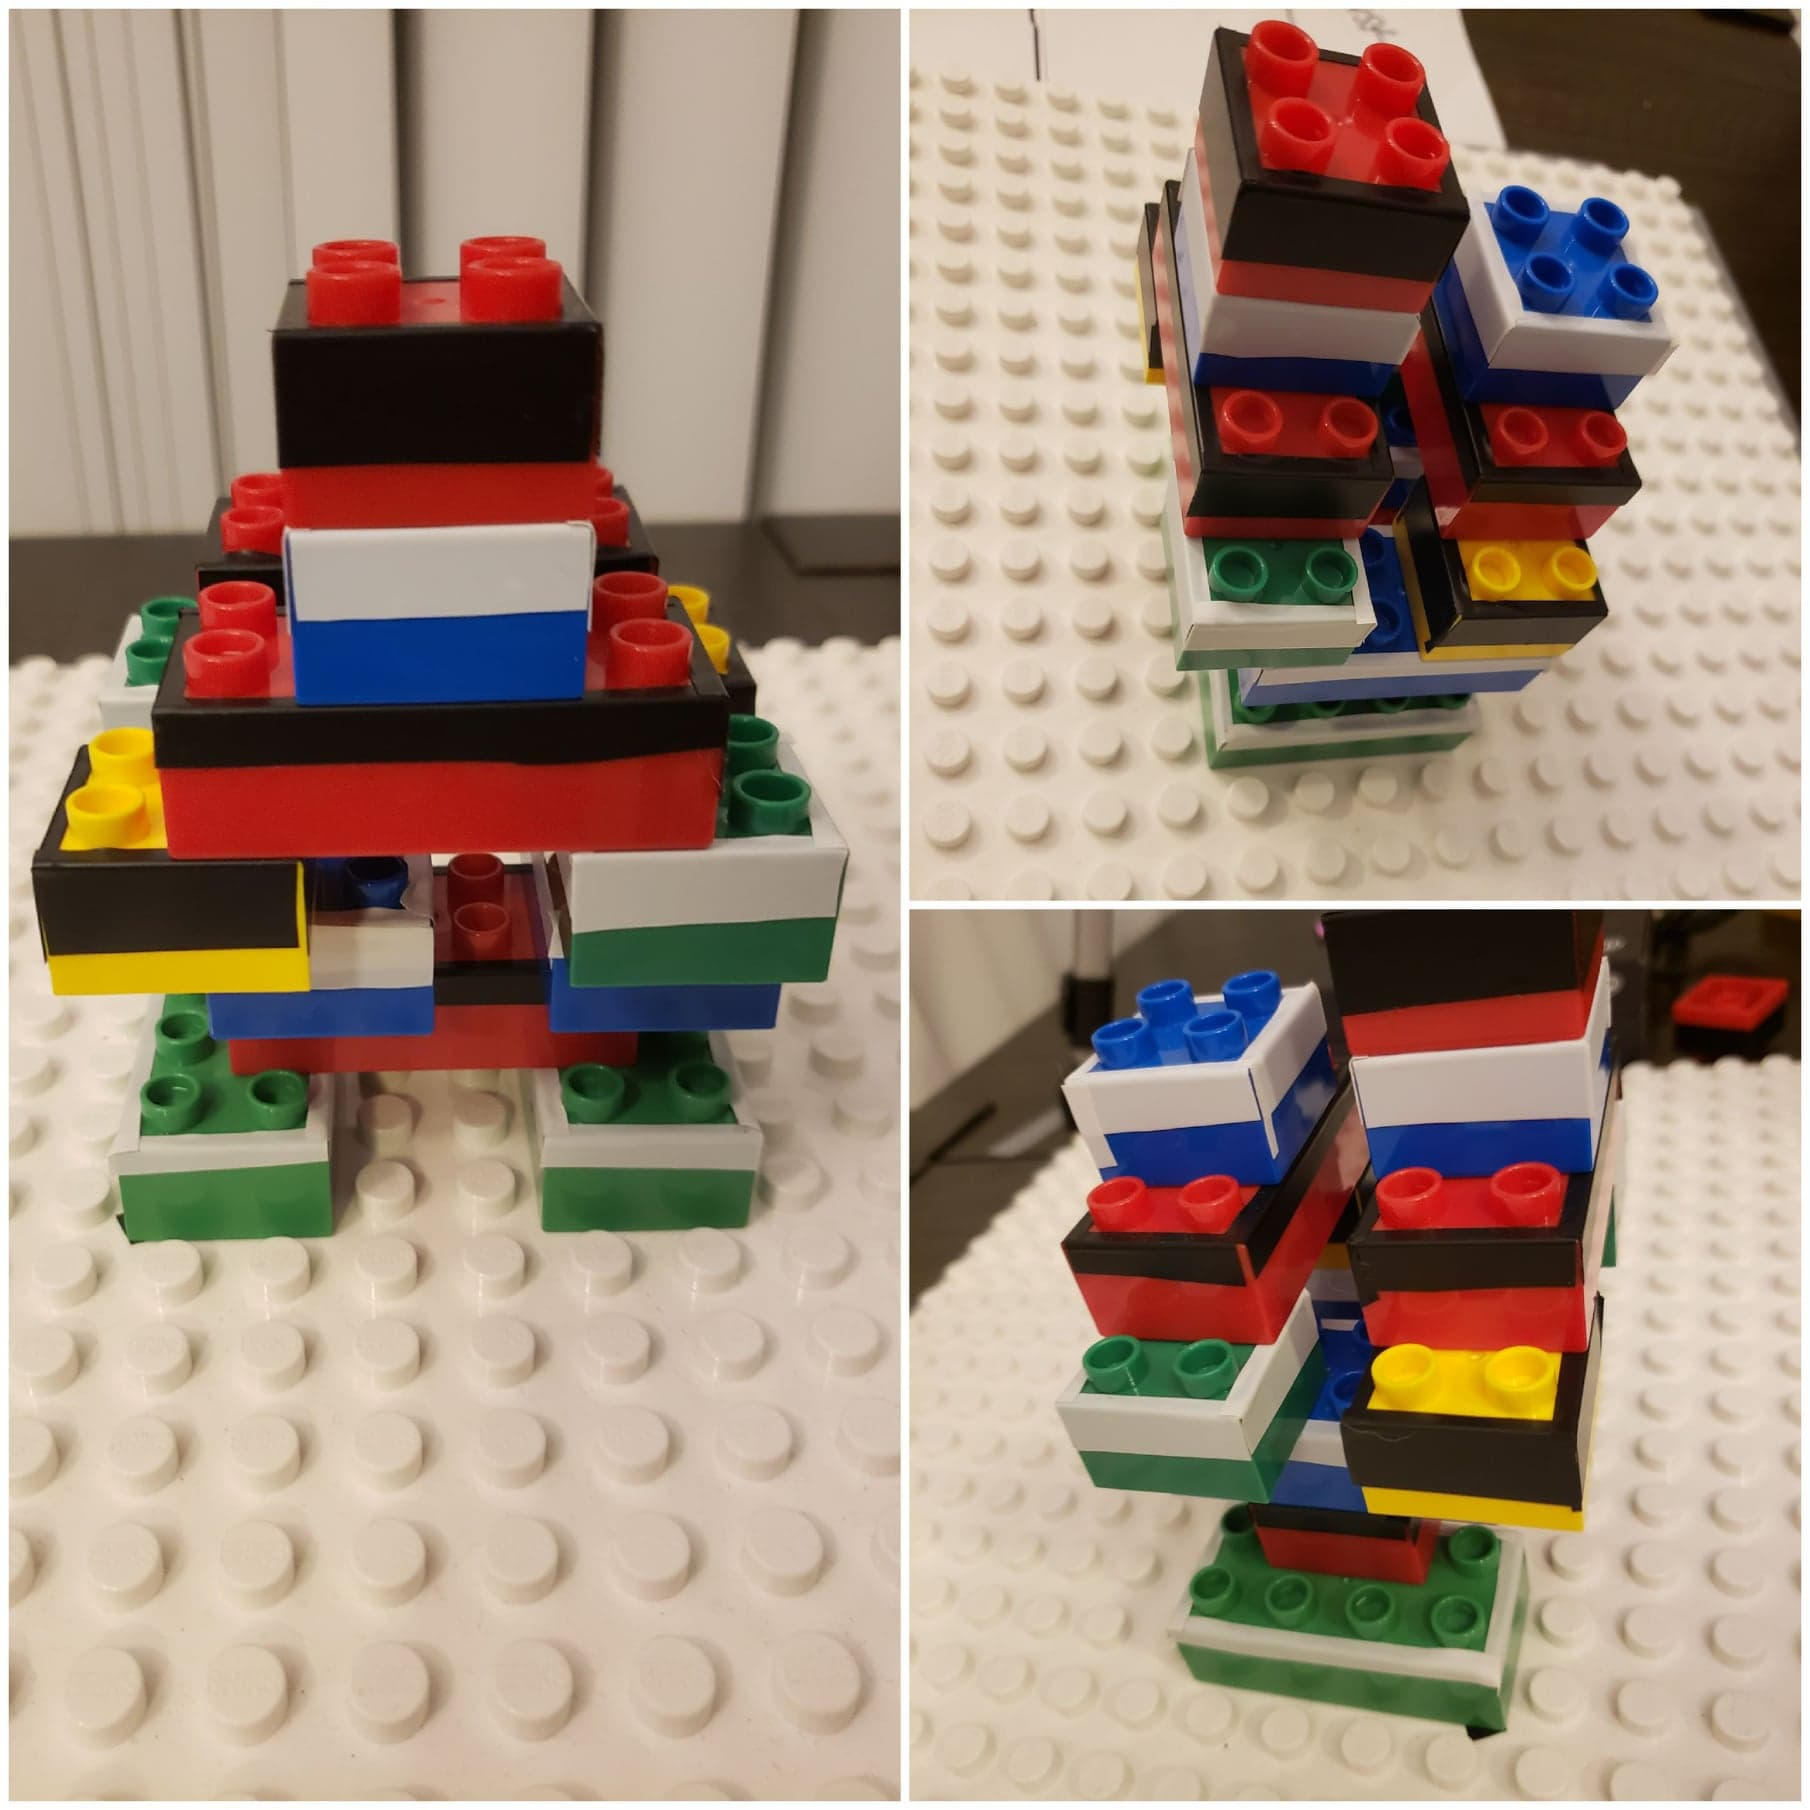
\includegraphics[width=0.8\linewidth]{figures/e3.jpg}
       
       \caption[{}]{\label{fig:fig_3-7a}}
    \end{subfigure}
    \begin{subfigure}{0.5\textwidth}
       \centering
    %   \includegraphics[width=\textwidth,height=\textheight,keepaspectratio]{fig_3-3}
       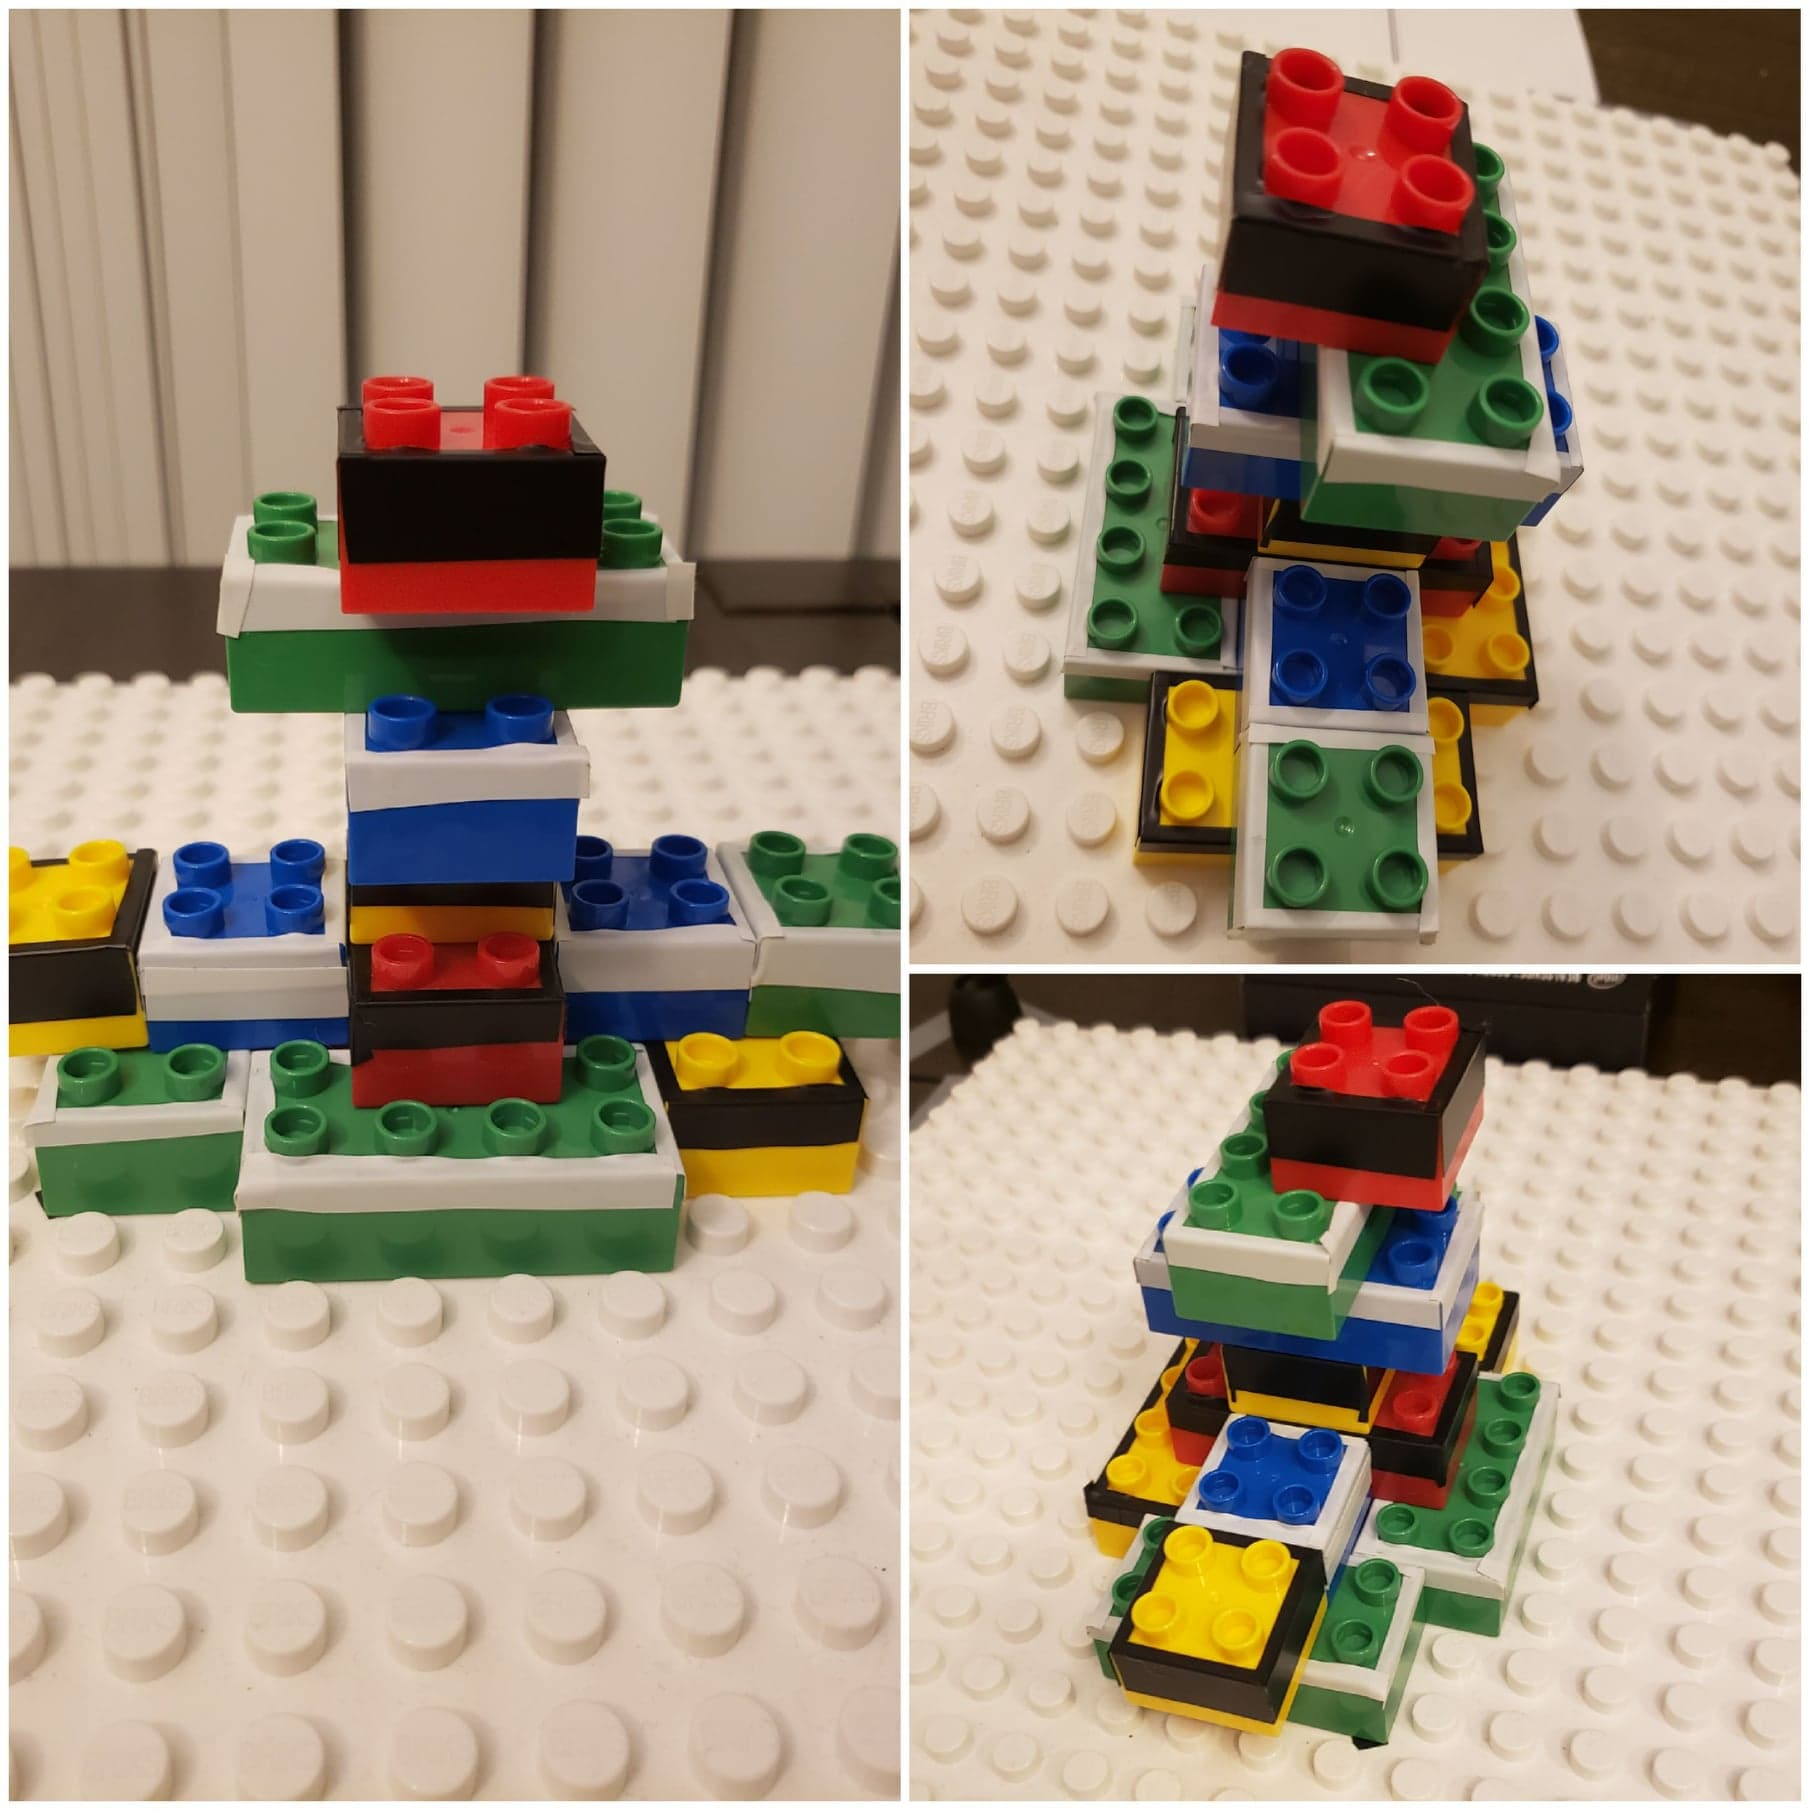
\includegraphics[width=0.8\linewidth]{figures/e4.jpg}
       
       \caption[{}]{\label{fig:fig_3-7b}}
    \end{subfigure}
    \begin{subfigure}{0.5\textwidth}
       \centering
    %   \includegraphics[width=\textwidth,height=\textheight,keepaspectratio]{fig_3-3}
       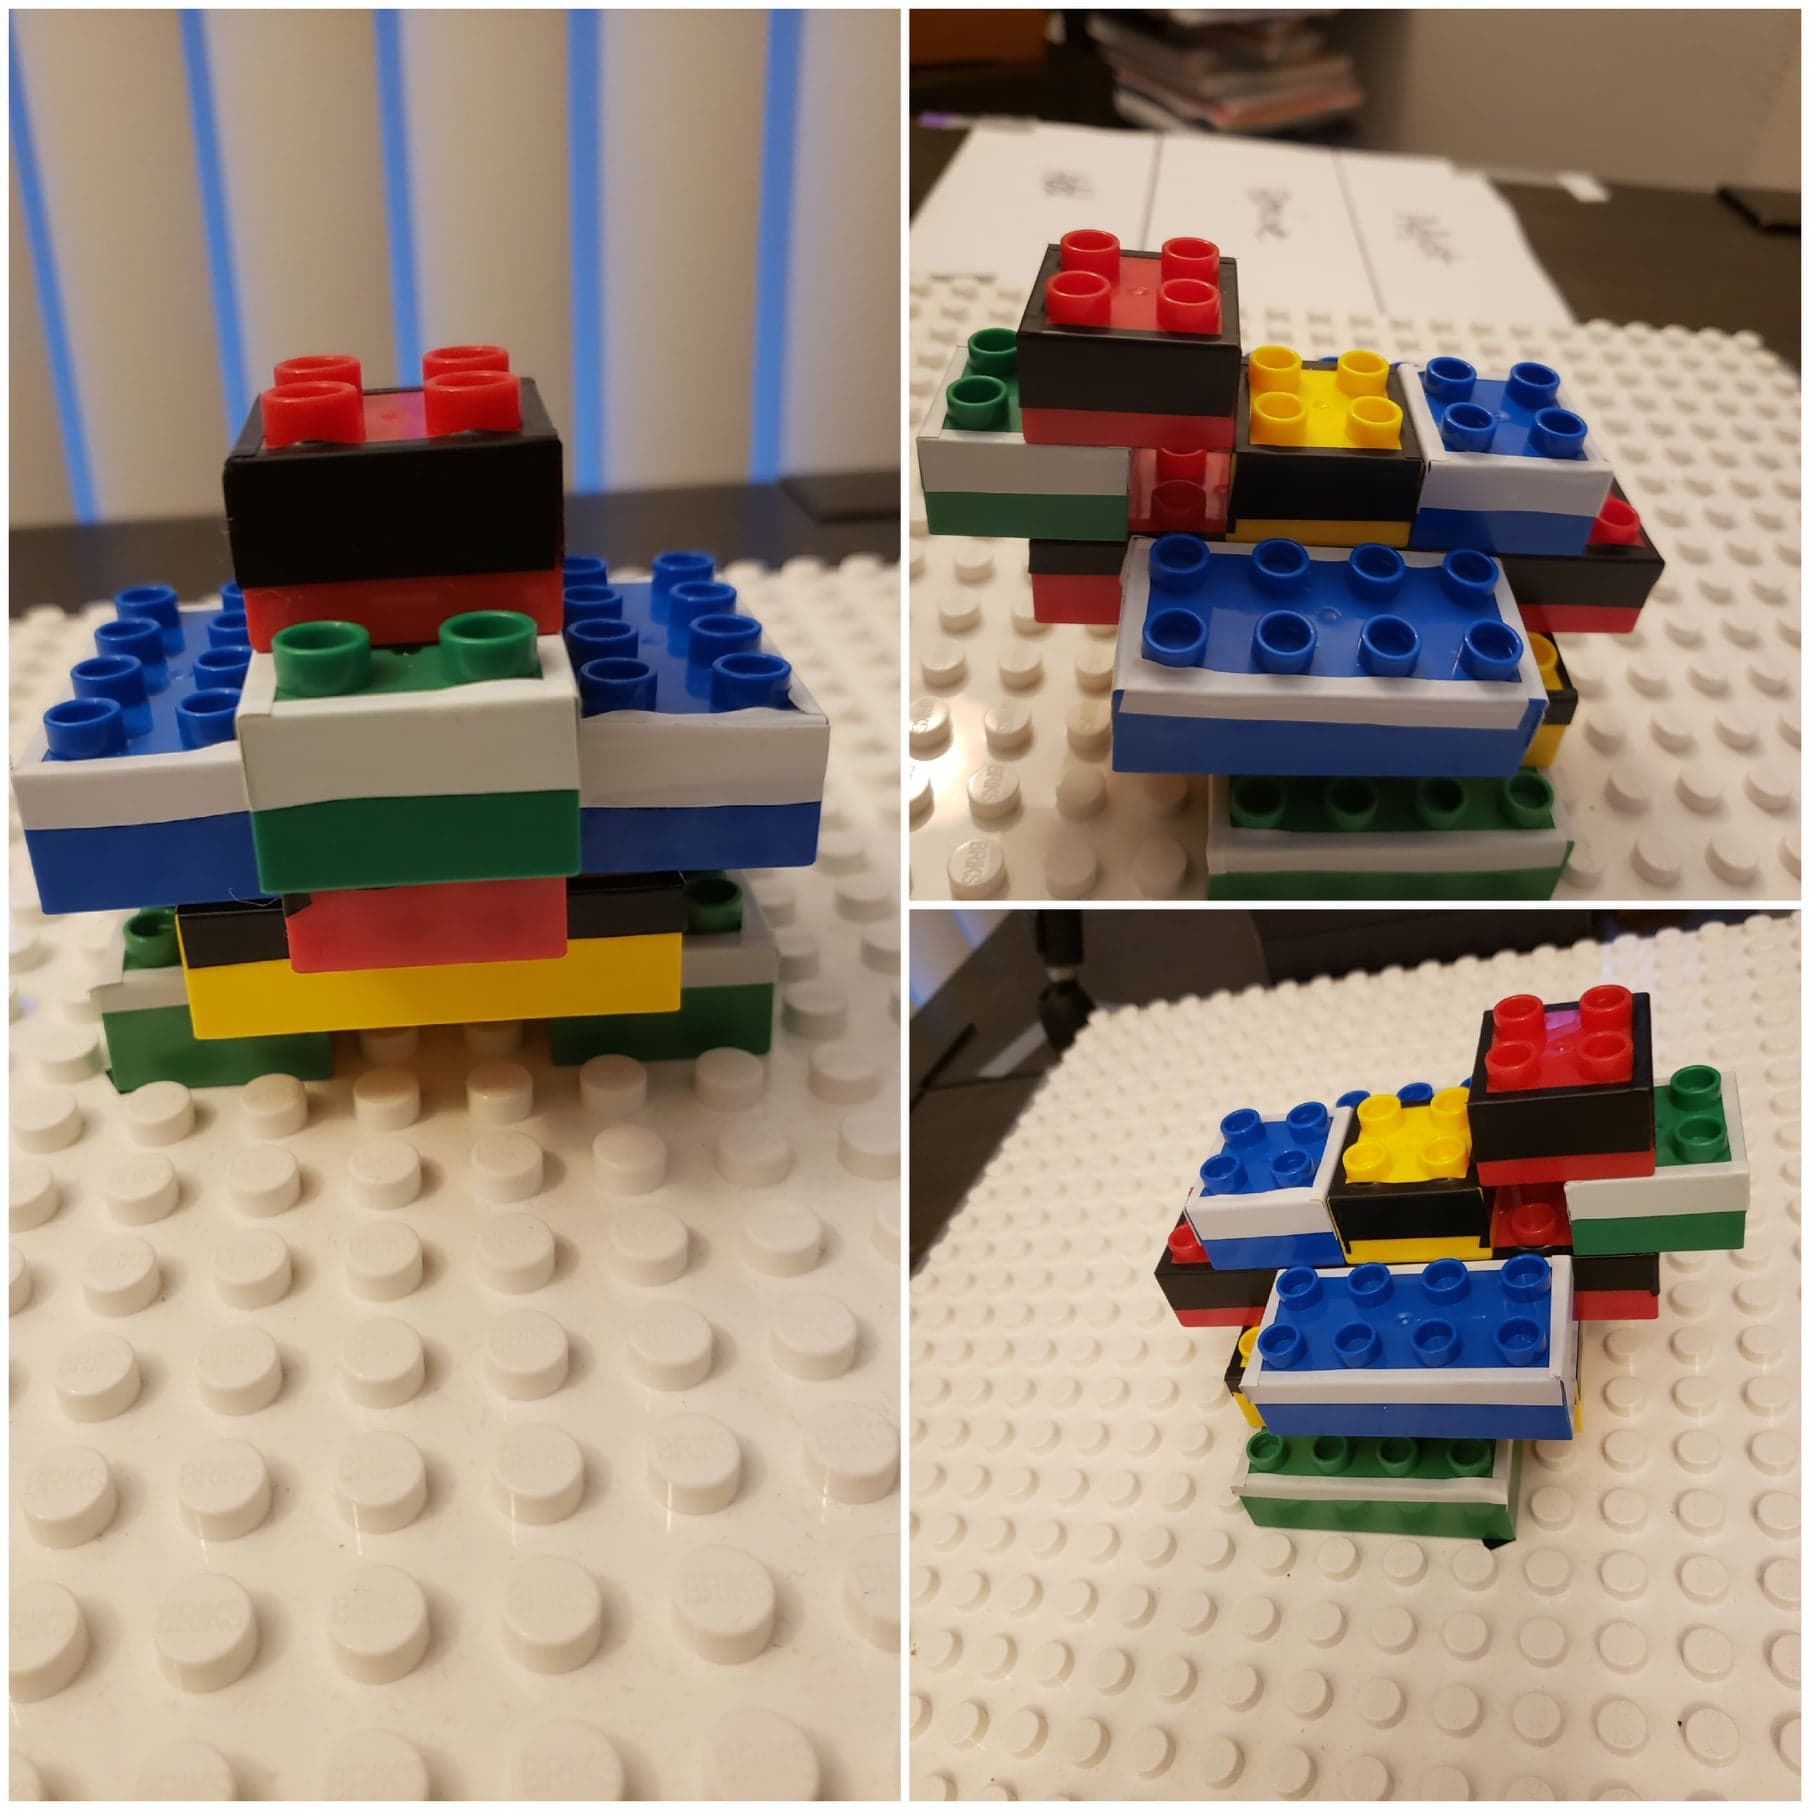
\includegraphics[width=0.8\linewidth]{figures/e5.jpg}
      
       \caption[{}]{ \label{fig:fig_3-7c}}
    \end{subfigure}
    \begin{subfigure}{0.5\textwidth}
       \centering
    %   \includegraphics[width=\textwidth,height=\textheight,keepaspectratio]{fig_3-3}
       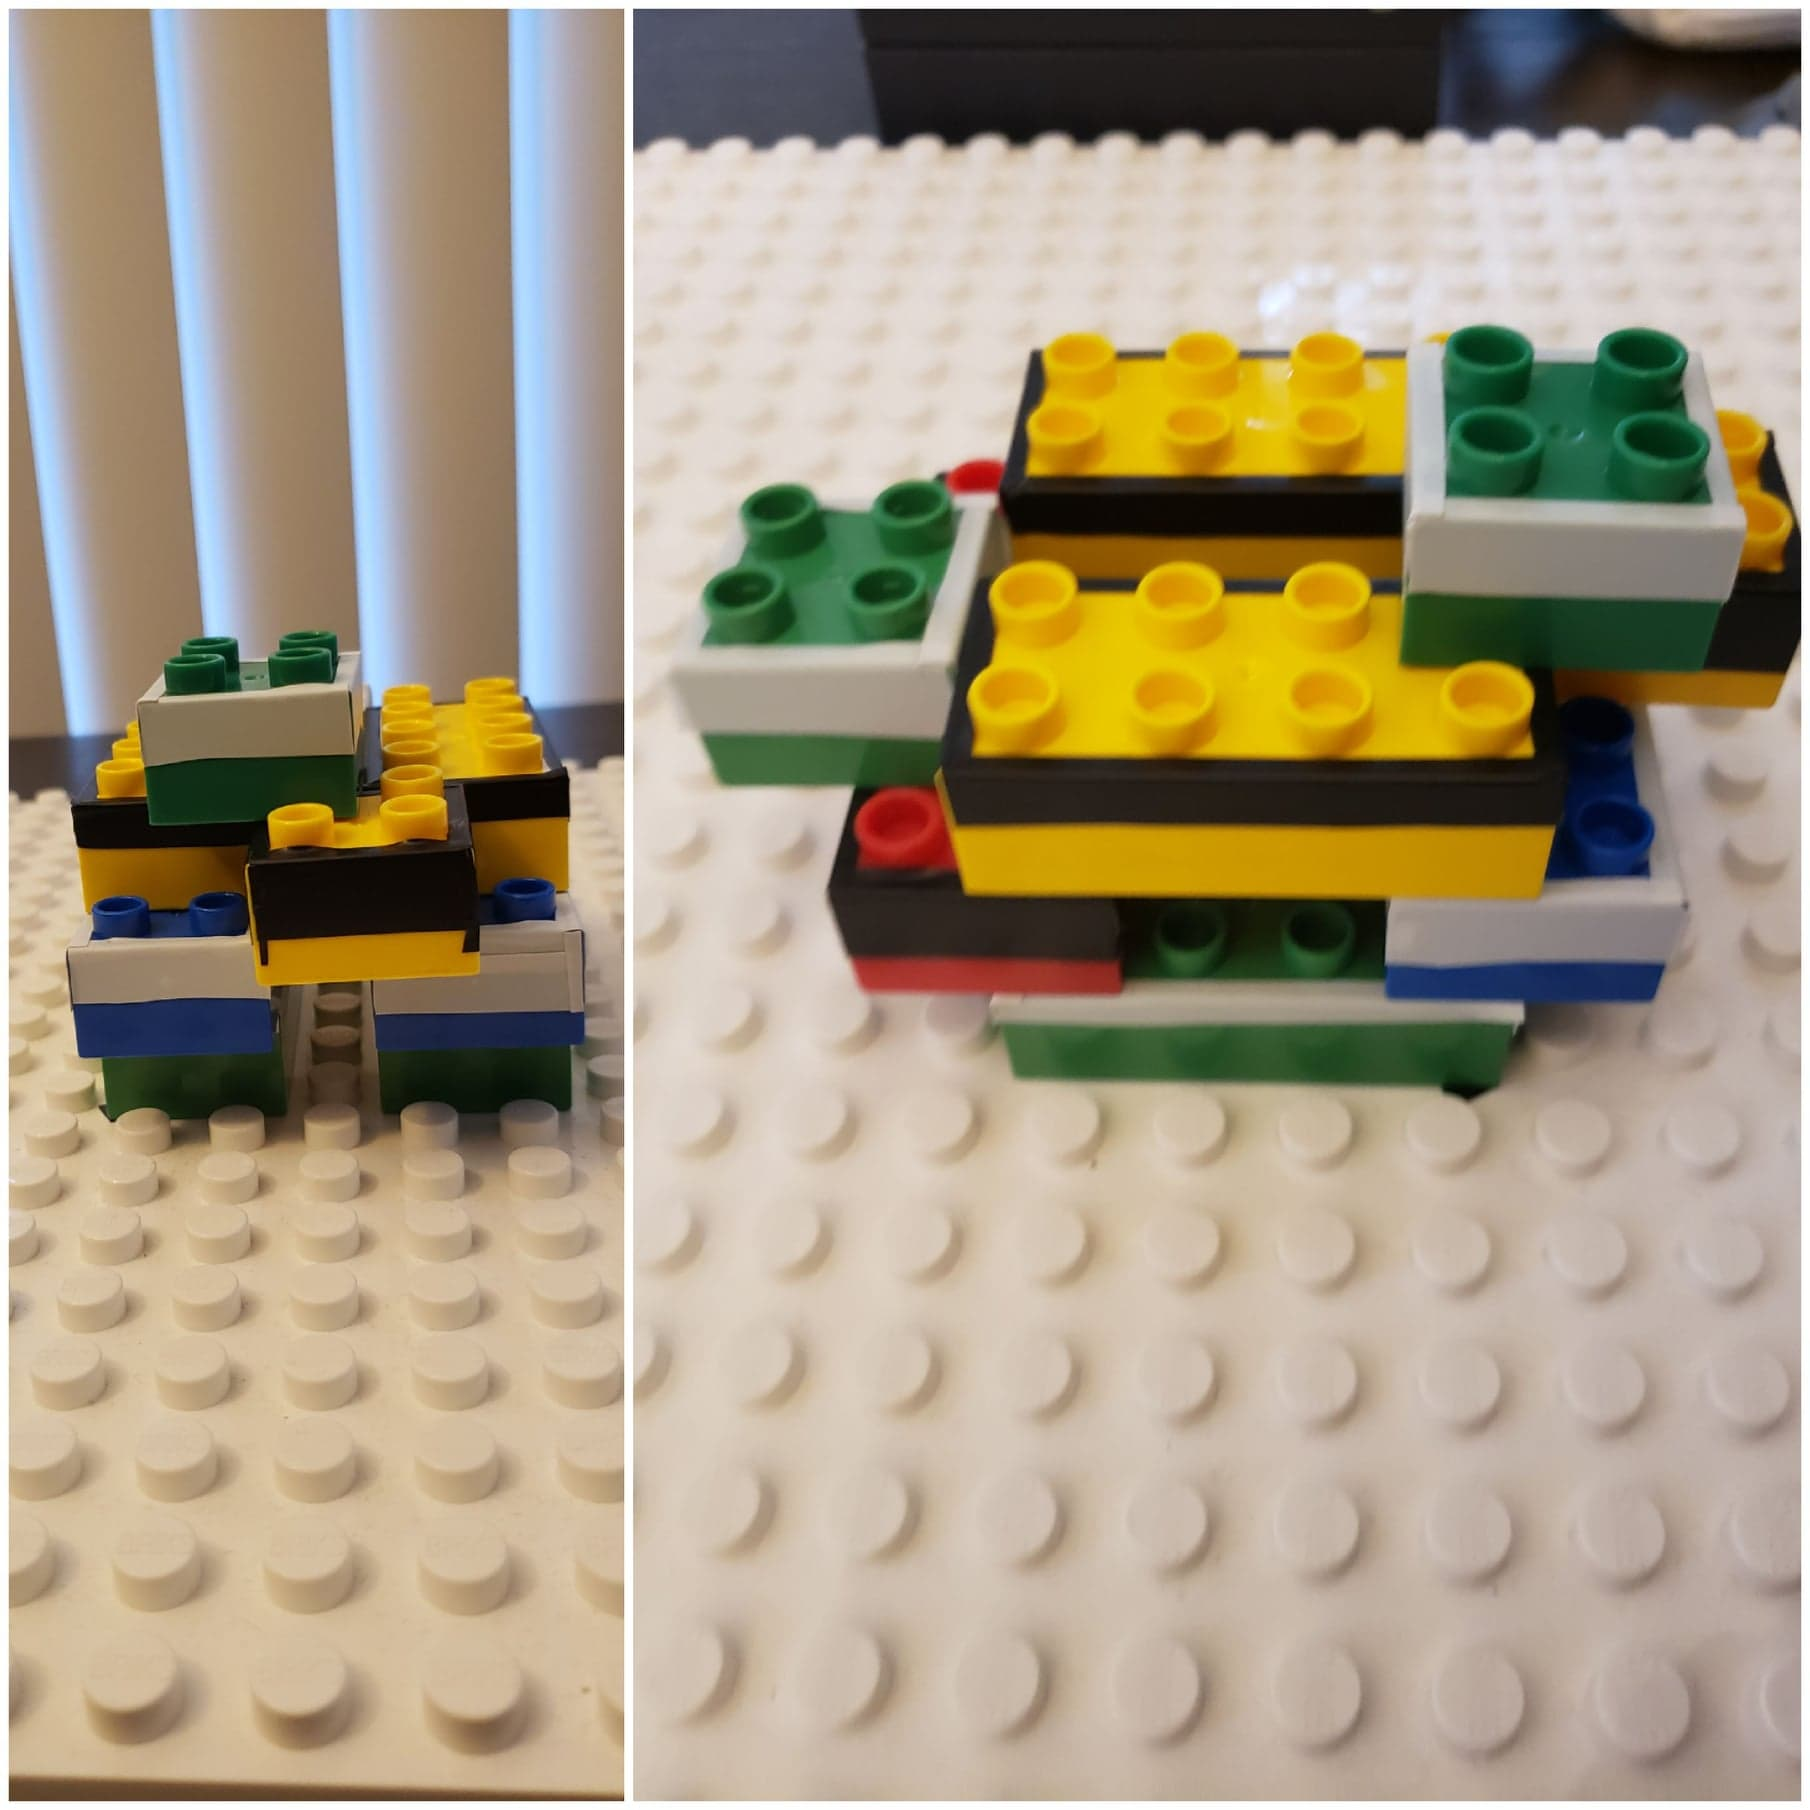
\includegraphics[width=0.8\linewidth]{figures/e6.jpg}
       
       \caption[{}]{\label{fig:fig_3-7d}}
    \end{subfigure}
    \begin{subfigure}{0.5\textwidth}
       \centering
    %   \includegraphics[width=\textwidth,height=\textheight,keepaspectratio]{fig_3-3}
       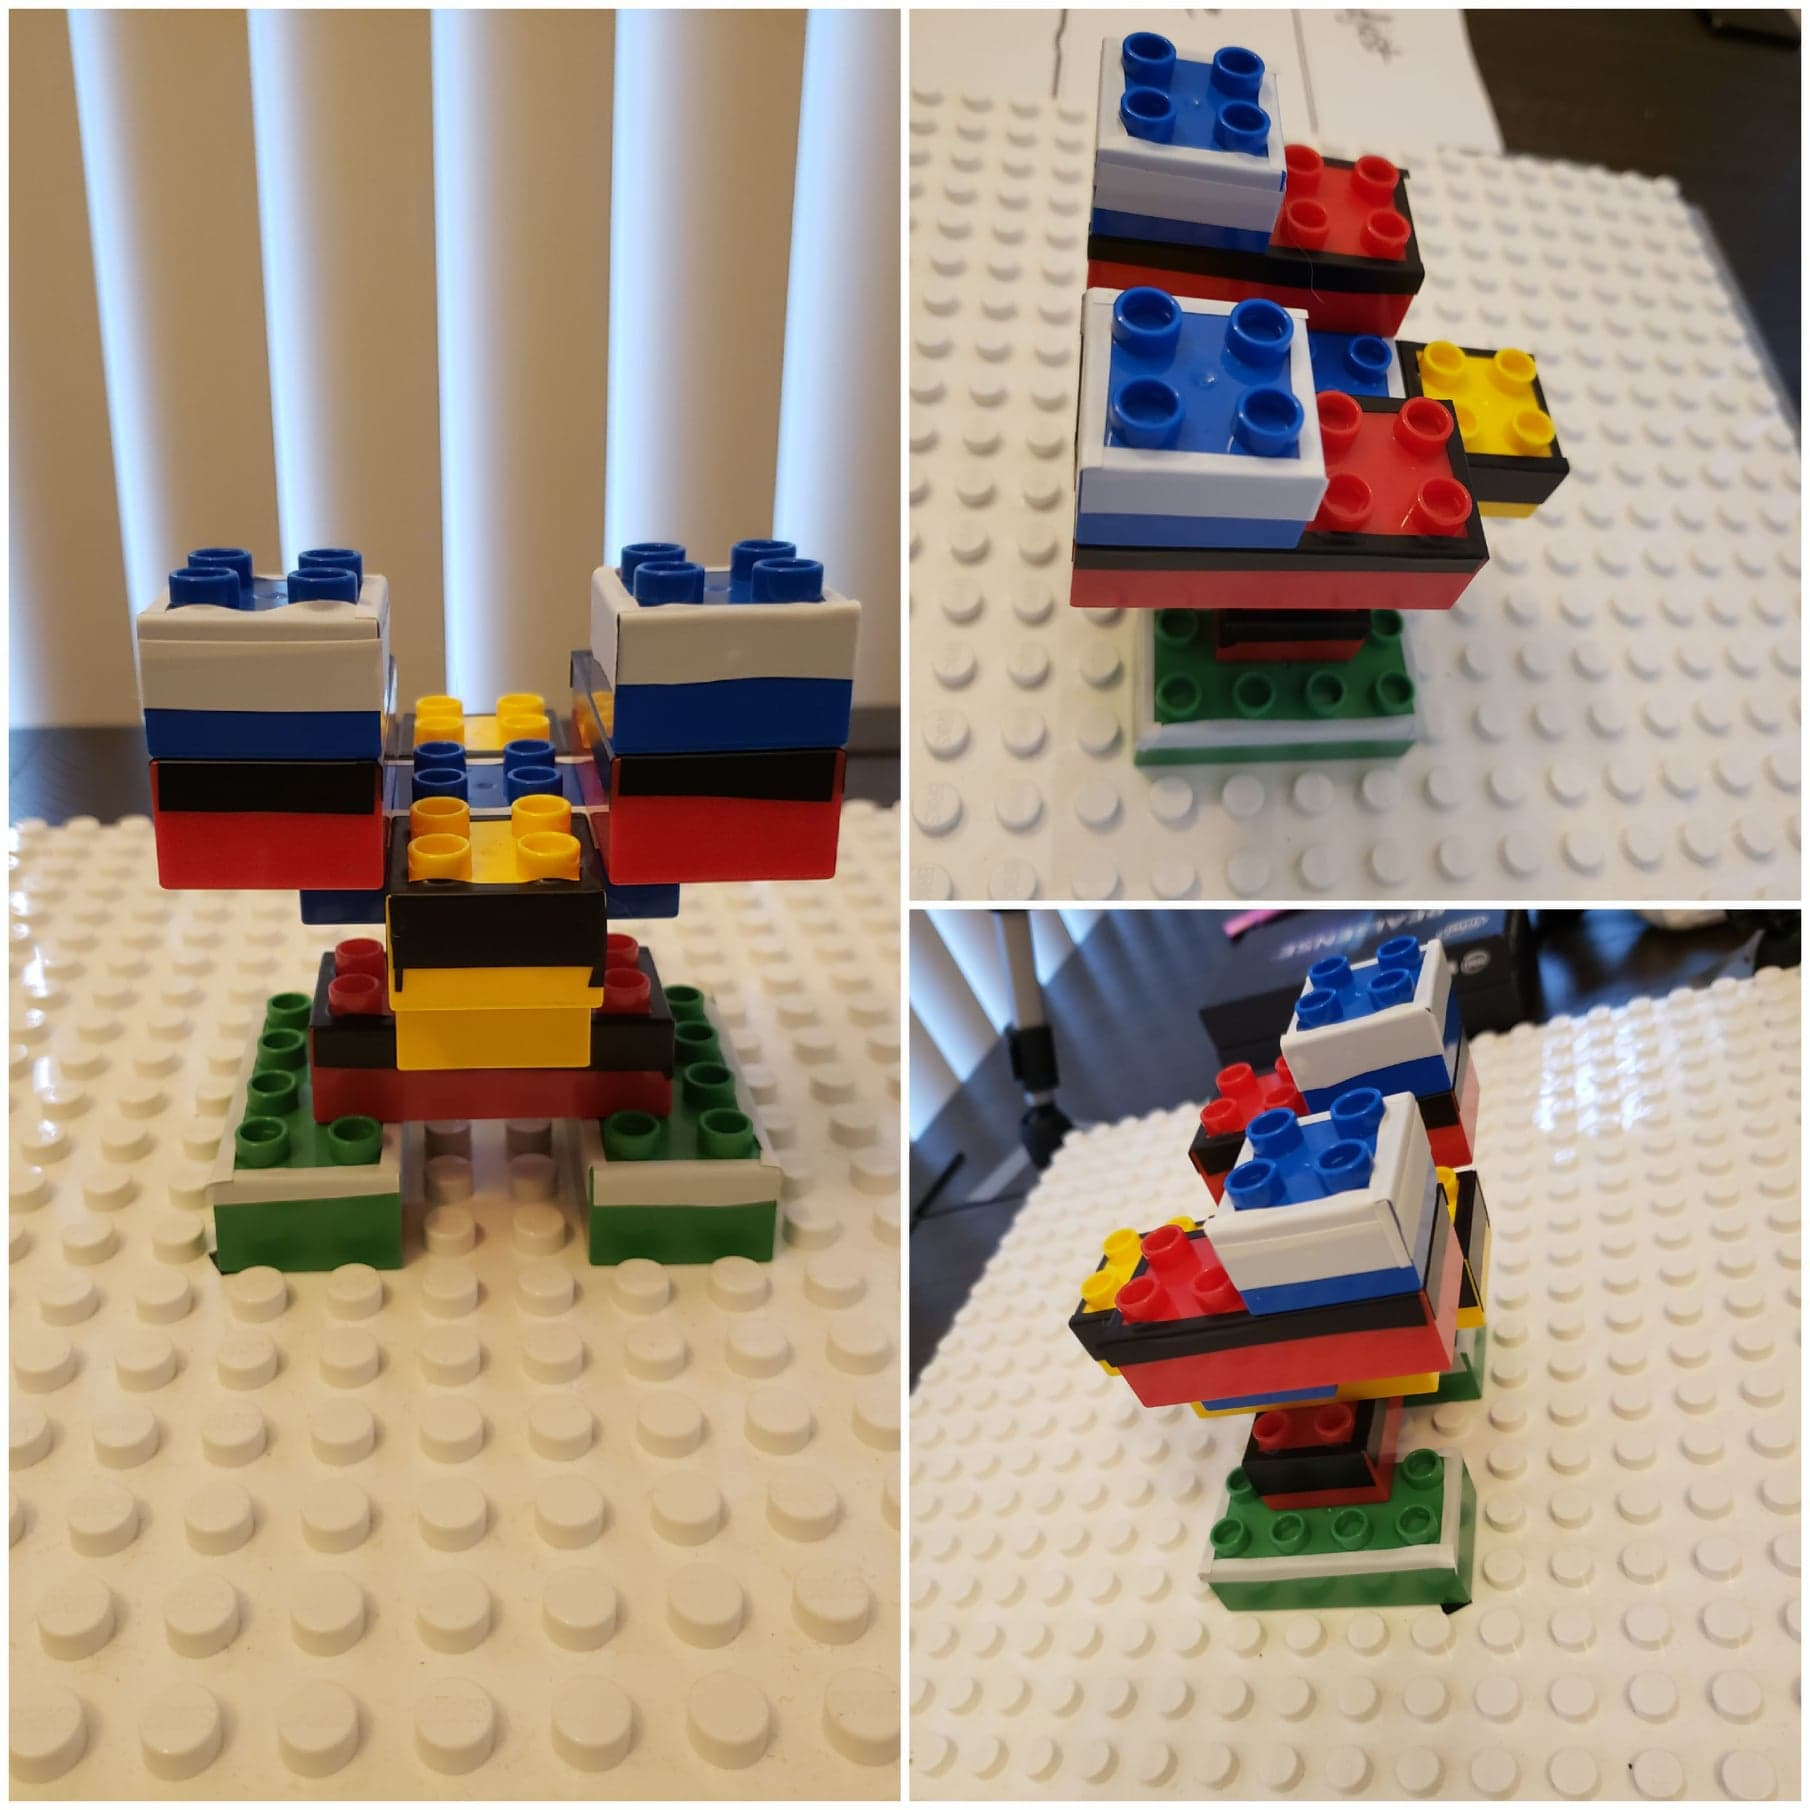
\includegraphics[width=0.8\linewidth]{figures/e7.jpg}
      
       \caption[{}]{ \label{fig:fig_3-7e}}
    \end{subfigure}
    \caption[{Complex 3D structures}]{Complex structures successfully completed in both learning and teaching modes. Picture on left is front view and picture(s) on right are side view(s).}
   \label{fig:fig_3-7}
\end{figure}
\subsect{Evaluation and Limitations}
The system runs on Ubuntu (in dual boot with windows) in real-time on a laptop PC with 5-core 2.3 GHz Intel\textsuperscript\textregistered{} processor. It takes about 2-5 seconds to update the model when required. There is no lag in the system. The system works fairly well in most of the cases. Some simple structures, which can be recreated by looking at only one view, were successfully completed by us in the learning mode and tested in teaching mode as shown in figure \ref{fig:fig_3-6}. Some complex structures were also tested by the system are shown in figure \ref{fig:fig_3-7}. These complex structures requires at least pictures of 2 views to recreate. These structures were successfully detected and stored by our system. Various random structures were also tried to look for possible errors and limitations of the system. Some of the errors and limitations observed are:

\begin{enumerate}
    \item Occlusion: Since only one camera is used to track the workspace, if the block to be added or removed is not fully seen by the camera, it will go undetected and cause errors as shown in figure \ref{fig:fig_3-4}. Using multiple RGB-D streams from various cameras can eradicate this issue. 
    \item Confusion: As explained above, the error in \textbf{.z} is fixed by intuitively lowering the level until it overlaps at least one block underneath it. This fixes the \textbf{.z} for time being for that block but when new block of same shape (or appearing to be of same shape) is requested to be added, the overestimated z would stop at a level higher than before thus re-adding that object thinking that it is a new object at upper level as shown in figure \ref{fig:fig_3-5}. Using better method for estimating error in depth because of oblique camera or using multiple RGB-D cameras can help reduce this error.
    \item Due to changes in light source, sometimes, HSV based color detection is faulty but it can be fixed by fixing the light source.
    \item The whole 3D structure is grounded on a base, thus not allowing the user to move it around in space. 
    \item The blocks have been taped on edges (as seen in figures) to assist color segmentation and enable differentiation of same colored blocks. The boundaries allow different shapes and multiple blocks of similar characteristics to be used for block building. 
\end{enumerate}
\begin{figure}[h]
   \centering
%   \includegraphics[width=\textwidth,height=\textheight,keepaspectratio]{fig_3-4}
   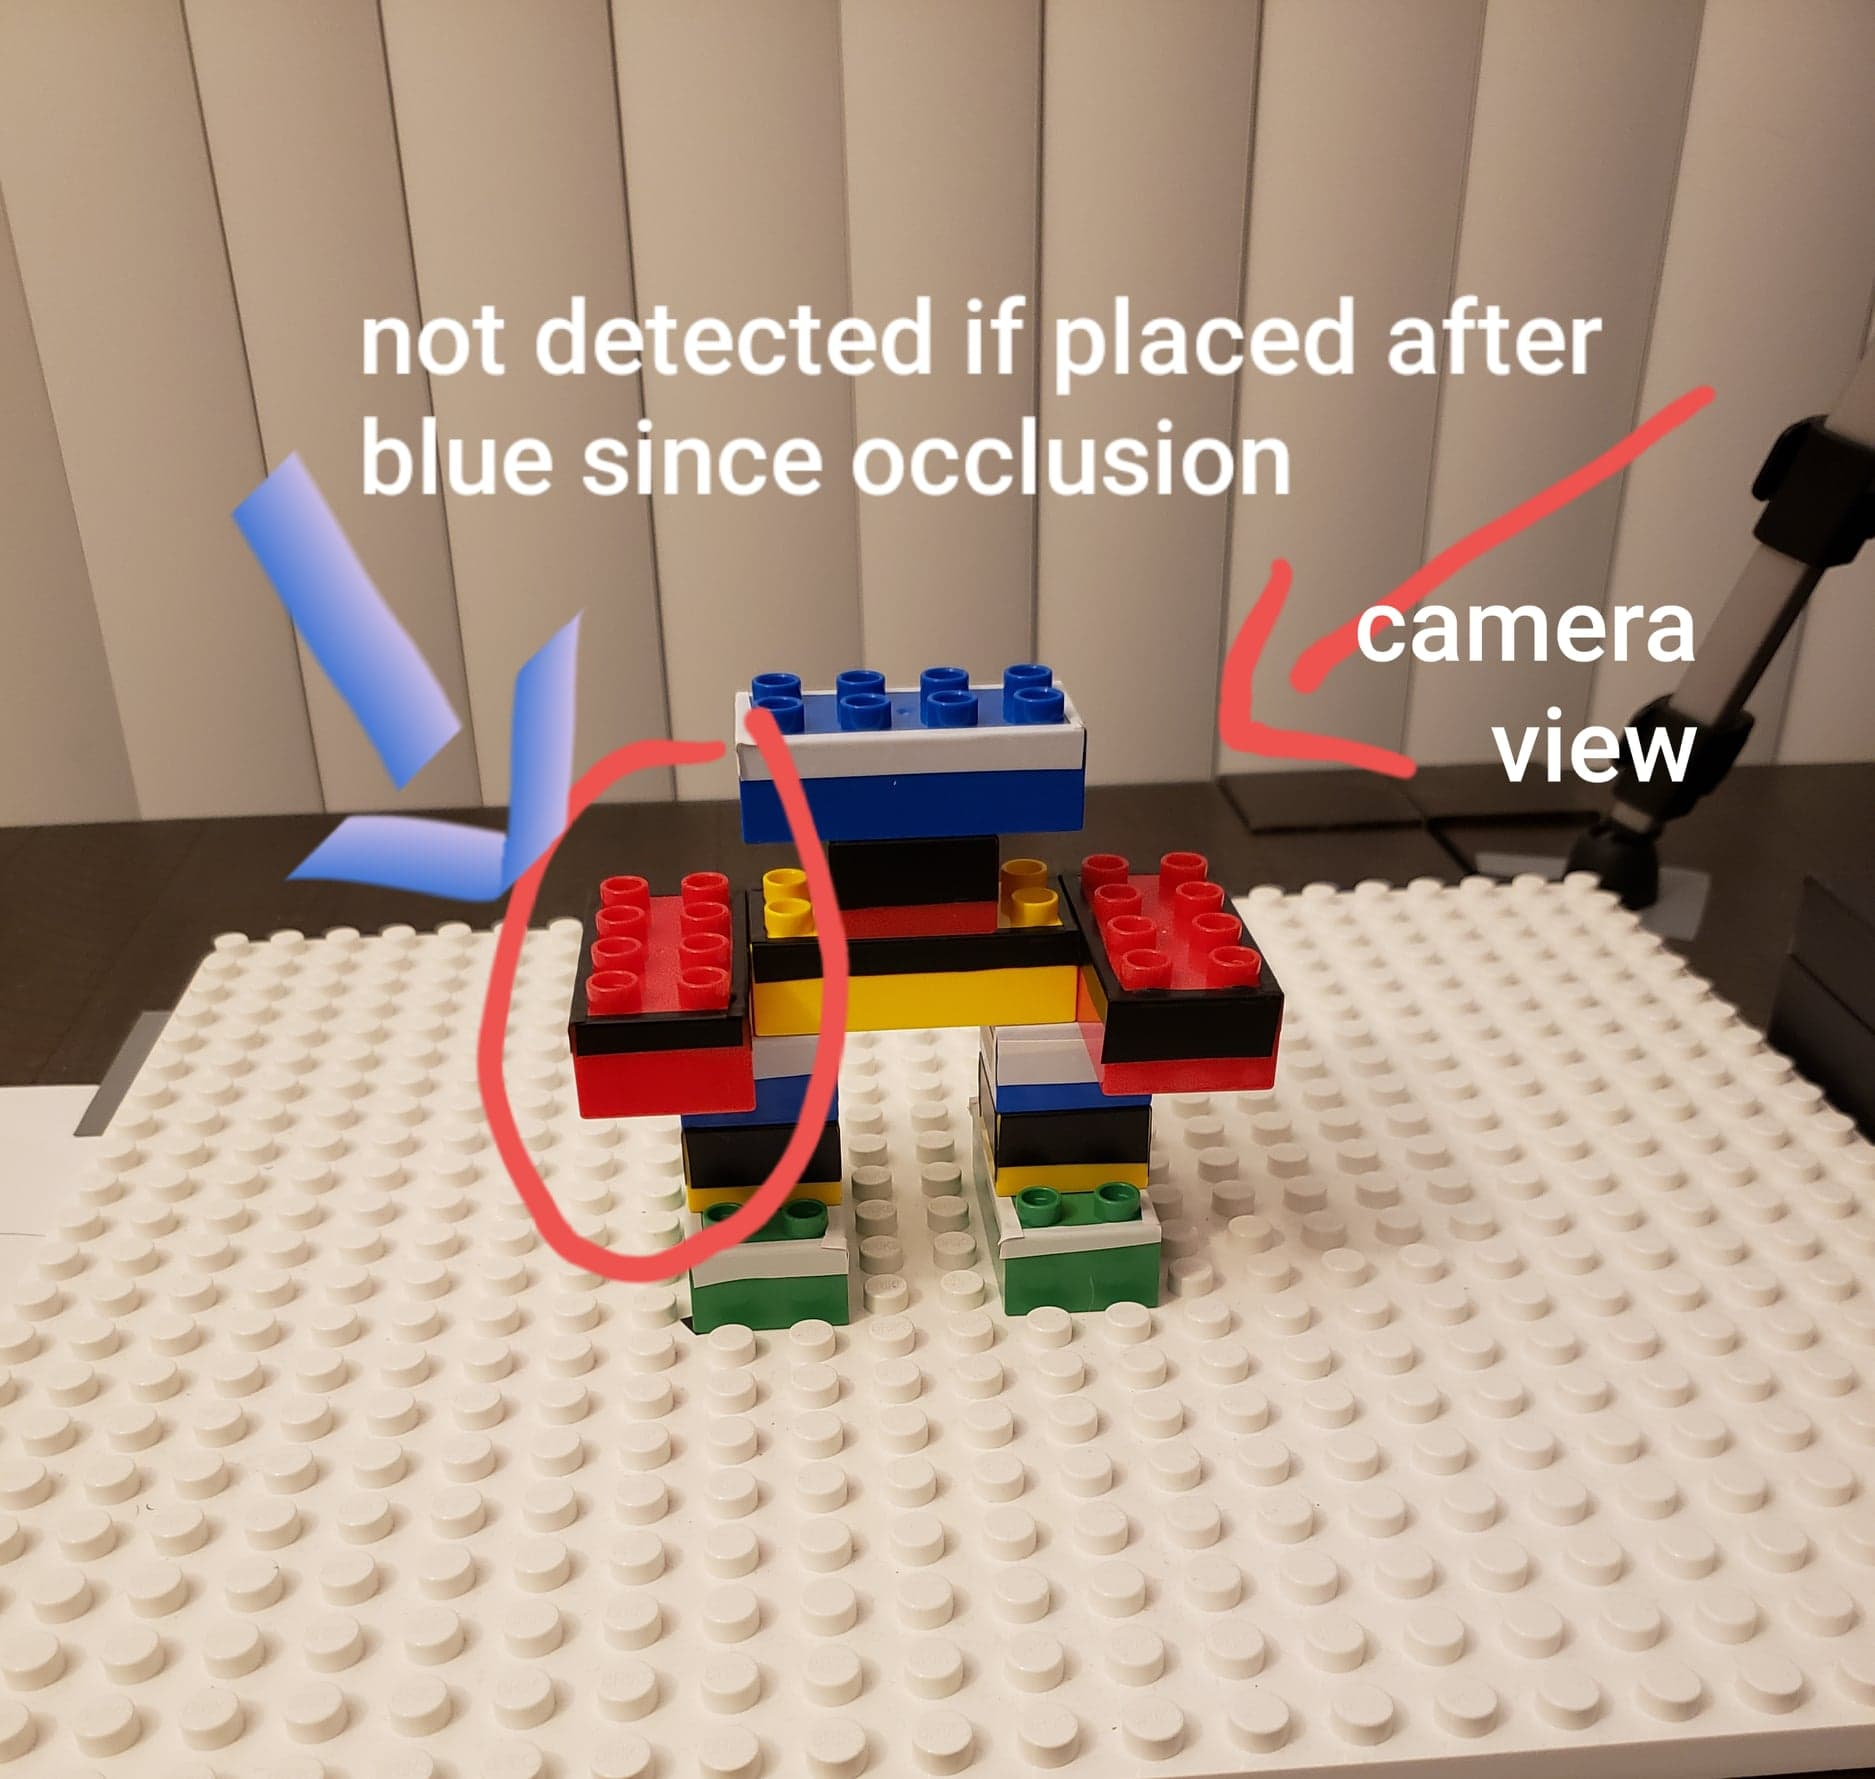
\includegraphics[scale=0.2]{figures/occlusion.jpg}
   \caption[{Example of occlusion}]{Example of occlusion: The circled $2 \times 4$ red block on level 4 will not be detected if placed after the $2 \times 4$ blue block on level 6 because the camera cannot see it fully}
   \label{fig:fig_3-4}
\end{figure}

% Figure 3-5
\begin{figure}[h]
   \centering
%   \includegraphics[width=\textwidth,height=\textheight,keepaspectratio]{fig_3-5}
   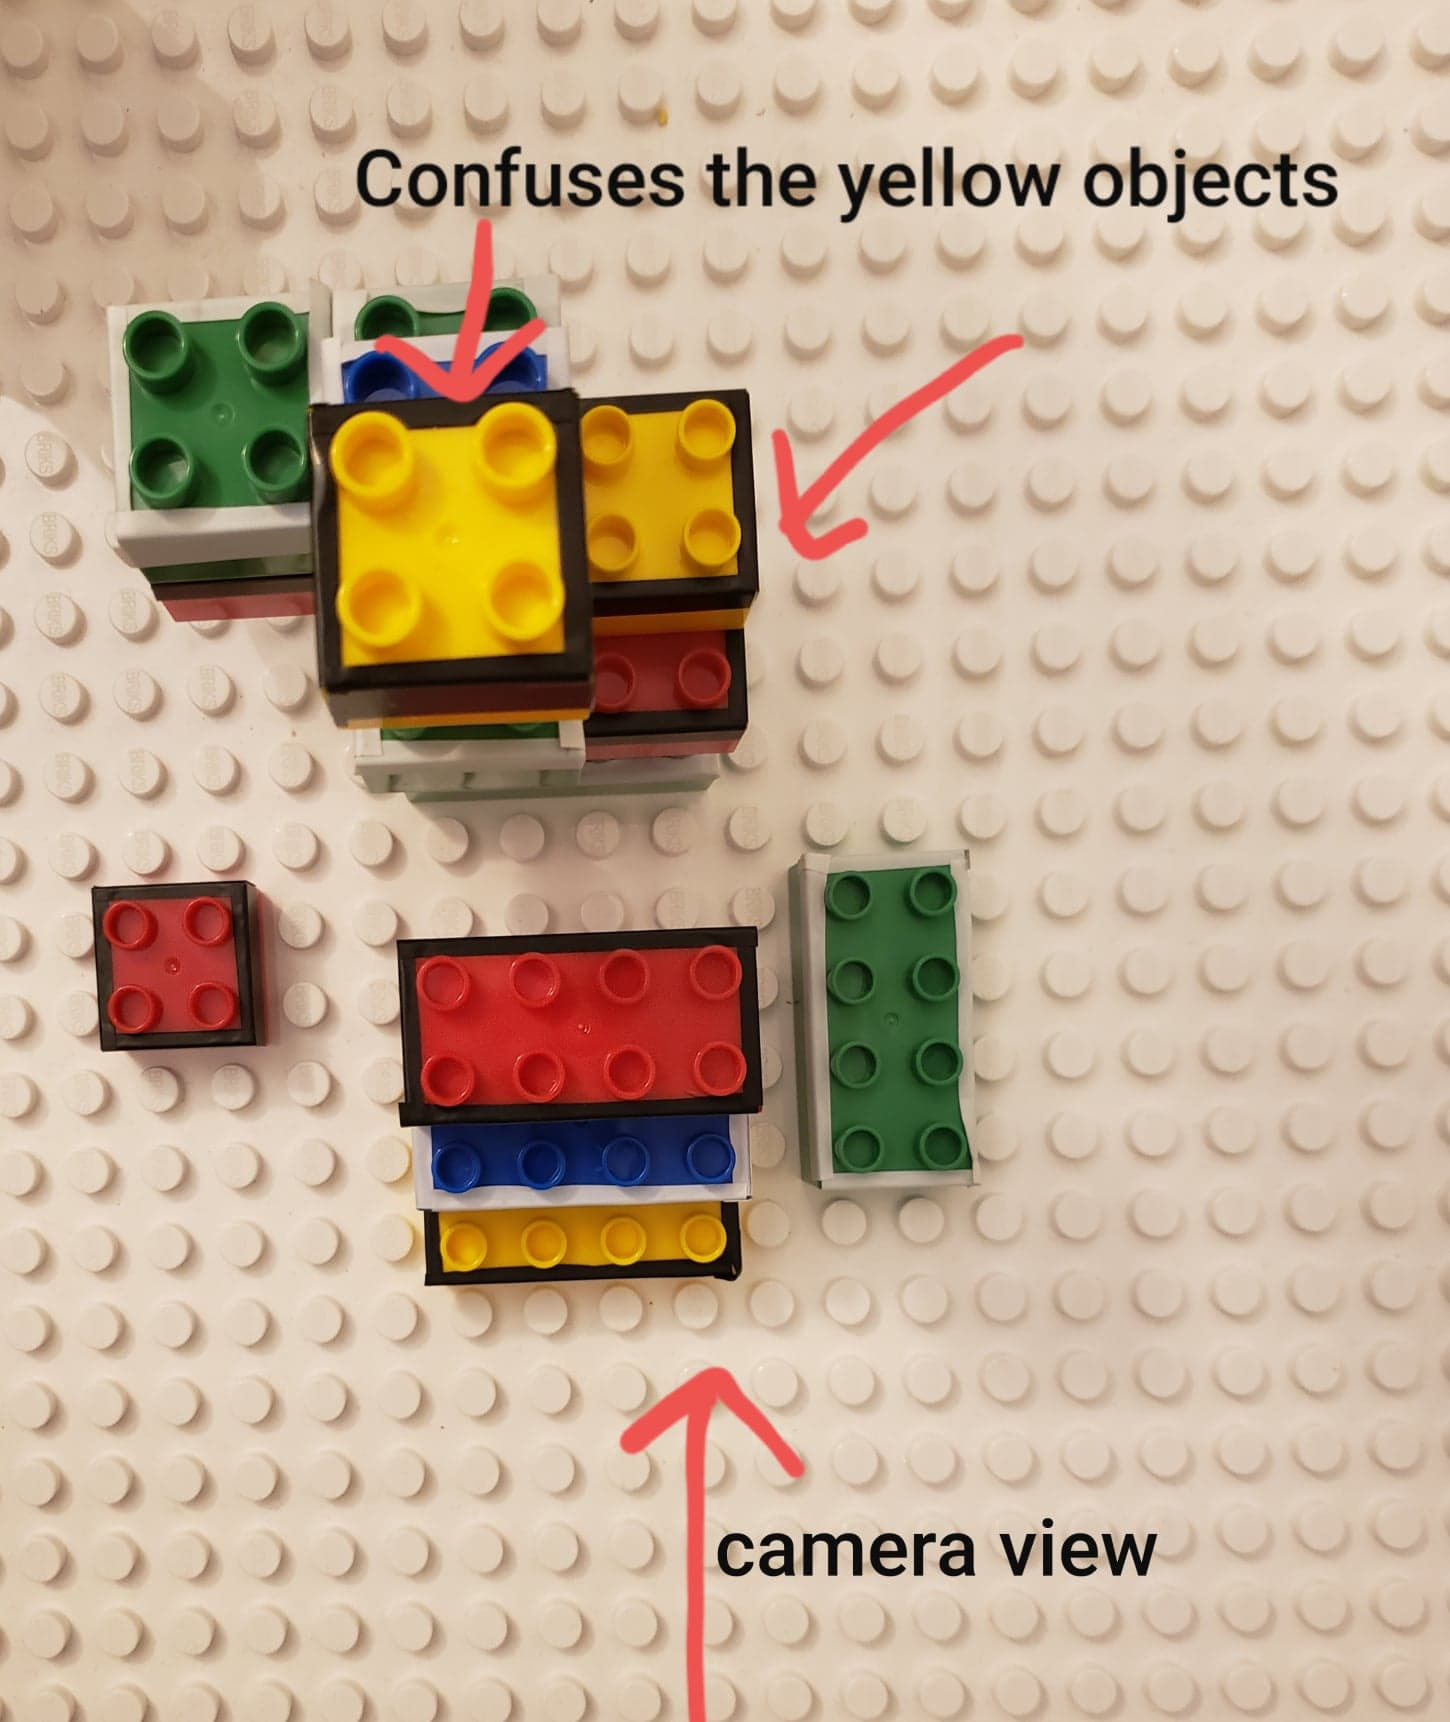
\includegraphics[scale=0.2]{figures/confusion.jpg}
   \caption[{Example of confusion}]{Example of confusion: The $2 \times 4$ yellow block at lower level is mistakenly added as a $2 \time 2$ yellow block because it appears to be a $2 \times 2$, even before the user placed the top level $2 \times 2$ yellow block because the rectangle at $\textbf{.z}=4$ originally had been assigned $\textbf{.z} > 4$ and it was corrected to 4. Thus, now the visible portion of lower level yellow block appears to be a new block added at level 5 ($\textbf{.z} = 5$)}
   \label{fig:fig_3-5}
\end{figure}
Despite these limitations, the proposed perception module has some advantages over similar systems. It is able to use two different shapes unlike in Gupta and colleagues' system \parencite{gupta2012duplotrack} which uses only $2 \times 4$ blocks. It can be extended to other shapes e.g. $1 \times 2$ blocks easily. Also, it is able to use multiple blocks of 4 colors of 2 shapes unlike Jones and colleagues' system \parencite{jones2019toward}  which uses only one block of each shape ($2 \times 4$ and $2 \times 2$) and 4 colors (total of 8 blocks). Our model representation is robust and efficient. Such simple representation enables us to track an assembly which has multiple paths towards correct solution. We are able to get all possible correct next actions and all possible removable items at any step. It is not a step by step process strictly since there can be multiple correct actions at any step unlike step by step guided system proposed by Gupta and colleagues \parencite{gupta2012duplotrack}. Also, we use a reference block for defining (0,0) for xy-coordinates, thus, the learnt graphs stay valid even if the reference block is moved at the start of each 3D building task.  


%\subsect{Applications}


\sect{Feedback}
Second module of the system is providing feedback in teaching mode to help the user finish the 3D block building task at hand. Feedback system receives various types of errors in new block from each possible correct block. Based on the number of possible correct blocks, number of errors from each possible correct block and type of errors, the error on which the robot must give feedback is decided. Following rules are followed:
\begin{enumerate}
    \item If there is a possible correct block with 0 errors from new block, a brief statement confirming the correctness of the action and suggesting to continue is provided. We call these statements \emph{continuers}. 
    \item If there is only one possible correct block and there is only one type of error, that error is selected by default.
    \item If there are two or more errors with respect to the only possible correct block, following priority is considered while choosing the error to respond to:\\
    Error in: Shape $>$ Color $>$ Orientation $>$ Level $>$ Position
    \item If there are two or more errors with respect to two or more possible correct blocks. The possible correct block with which there are least errors is selected and the error priority is decided as following:\\
    Error in: Shape $>$ Color $>$ Orientation $>$ Level $>$ Position
\end{enumerate}
Two main questions to answer are: When to give feedback and what would the feedback statement say. As far as \emph{When} is concerned, for this exploratory study we provide feedback to user every time a mistake is made. Although due to delays in execution of robot behaviour continuers might be skipped every now and then. To answer the second question, we inspire from feedback strategies that are summarized in table \ref{tab:tab_2-1}. Table \ref{tab:tab_3-1} shows the design of feedback statements that is published to a rostopic for robot to convey to the user. 
\begin{table}[]
    \centering
\begin{tabular}{ | m{2cm} | m{3cm}| m{8cm} | } 
\hline
\textbf{Error type} & \textbf{Feedback Type} (refer to table \ref{tab:tab_2-1}) & \textbf{Feedback Statement} \\ 
\hline
\multirow{4}{4em}{Shape or Color}  & 8a. & The shape/color should be \_ instead of \_ \\ \cline{2-3}
& 1. 7c. 8b. & Hmm, are you sure you need a \_ here? \\ \cline{2-3}
& 3. 4. 7c. & So, if this is a \_ , what should be the next step?\\ \cline{2-3}
& 7c. 8b. & What if we try a \_ instead?\\ \cline{2-3}
\hline
\multirow{3}{4em}{Orientation}  & 8a. & The orientation is wrong. You need to rotate the block \\ \cline{2-3}
& 1. 8b. & Umm. Does this orientation looks right to you? \\\cline{2-3}
& 7d. 7h. 8b.  & What if we rotated the block, Wouldn't it look better? \\
\hline
\multirow{3}{4em}{Level}  & 8a. & The level is wrong. Move the block to upper/lower level. \\ \cline{2-3}
& 3. 8b. & What if we moved the block to upper/lower layer?\\ \cline{2-3}
& 7c. 8b. & Hmm, would you check if the block is at the right height?\\ 
\hline
\multirow{4}{4em}{Position}  & 8a. & The position is wrong, Move the block \_.  \\ \cline{2-3}
& 1. & I think the block is not at the right position. Would you try fixing it?\\ \cline{2-3}
& 7d. 7h. & Hmm, Let's try moving this block around a little bit to see if we get it right.\\ \cline{2-3}
& 3. 4. 7c. & If this is the right position for this block, think what would be on top of it?\\ 
\hline
For all  & 7d. & Let's look at the given picture to see if this looks alright. \\ 
\hline
No error & 2 & One of following \emph{continuers} with a nod: Go on. Continue. Hmm. Good. Right. \\
\hline
\end{tabular}
  \caption{Feedback statements based on selected error and inspired from literature as summarized in table \ref{tab:tab_2-1}.}
    \label{tab:tab_3-1}
\end{table}

\sect{Robot Behaviour}
The third and last module of the system is introducing somewhat life-like movements in the robot. The robot we are using is Maki, a 3D printed robot with 7 servos and controlled using arbotix\_m controller as seen in the setup (figure \ref{fig:fig_1-1}. Maki provides verbal feedback when a mistake is made by the user. Microsoft\textsuperscript\textregistered{} Azure text-to-speech service is used to convert the feedback statement into human-like voice. Apart from speech, we program Maki to nod slightly to acknowledge the correct actions of user along with continuers such as \emph{go on}, \emph{continue} and \emph{good} etc. This is to remind user of its presence and keep the user engaged. We have implemented another robot behaviour known as referential gaze: In idle state, Maki looks at the user. When the user makes a mistake, the robot looks towards the play area as if it is analyzing the workspace, narrates feedback to the user and then looks back towards the user to take requisite action to correct the mistake made.















